\chapter{Анализ физических ограничений для решения задачи в ординарных и двойных каскадах}\label{ch:ch2}

Как уже было отмечено в главе \ref{ch1}, лишь некоторые из предложенных к настоящему моменту способов обогащения регенерированного урана потенциально способны решить задачу обогащения регенерата произвольного исходного состава в условиях одновременного выполнения ограничений на концентрации сразу нескольких изотопов и при заданном отношении между массой получаемого НОУ и исходной смеси регенерированного урана, поступающего для обогащения. В первую очередь, это касается разбавляющих схем на основе ординарного каскада. 
Однако, проведенный в главе \ref{ch1} теоретический анализ не позволяет априори определить при каких условиях может быть применена та или иная схема. В рамках настоящей главы кратко представлены результаты вычислительных экспериментов и сопутствующего им теоретического анализа, направленных на оценку возможности применения одиночных каскадных схем с разбавлением и двойных каскадов для получения обогащенного регенерированного урана в условиях многократного рецикла. 

\section{Модификации каскадных схем на основе ординарного каскада: методическая часть}\label{ch2_stat}

Вернемся к рассмотренным в Главе \ref{ch1} модификациям каскадных схем, основанных на ординарном каскаде (рисунок \ref{fig:diagram1ch3}), для обогащения регенерированного урана с одновременным разбавлением четных изотопов. Каждая из схем, представленных на рисунке \ref{fig:diagram1ch3} реализует один из возможных способов разбавления регенерированного урана. Отличия в способах состоят в том, в каком именно узле осуществляют разбавление регенерата, либо в  используемой в качестве разбавителя смеси. Например, в качестве разбавителя может выступать природный уран, НОУ из природного сырья.


\begin{figure}[ht]
  \centerfloat{\includegraphics[scale=0.7]{cascades/ord_all}}
  \caption{Схемы на основе ординарного каскада. Обозначения: $E$ -- поток питающего схему регенерата, $F_n$ -- поток разбавителя (природного урана или низкообогащенного урана); $W$ -- поток отвального ОГФУ тяжелого конца каскада; $P$ -- товарный низкообогащенный уран}\label{fig:diagram1ch3}
\end{figure}

Достоинства и недостатки подобных схем на теоретическом уровне подробно проанализированы в Главе \ref{ch1}. Однако, как следует из литературного обзора, для данных схем возможность их применения продемонстрирована, в первую очередь, на примере составов, характеризующихся относительно низким содержанием четных изотопов. Например, концентрация изотопа $^{232}$U в поступающем в обогащение регенерате составляет величину $1,5\cdot10^{-7}$\%, что в разы ниже значений, которые могут достигаться в условиях многократного рецикла (вплоть до $1\cdot10^{-6}$\%) \cite{palkinDesignanalyticalResearchRefinement2010}. Кроме того, при рассмотрении подобных каскадных схем, как правило, исходят из того, что уровень обогащения $^{235}$U регенерата или разбавителя в них, не превышает 10\%. В связи с этим представляется целесообразным проведение дополнительного исследования, которое бы позволило изучить взаимосвязи параметров модификаций каскадных схем обогащения регенерата на основе ординарного каскада при различных условиях. В свою очередь, это позволит оценить потенциал таких каскадных схем для обогащения регенерированного урана при различных внешних условиях. 

Таким образом, основная цель описанных ниже вычислительных экспериментов -- оценить возможности рассматриваемых модификаций ординарного каскада для обогащения регенерированного урана в условиях заметных (до одного порядка) колебаний концентраций четных изотопов, что характерно для его многократного рецикла. Рассмотрены случаи обогащения регенерированного урана двух составов с различным исходным содержанием чётных изотопов (см. таблицу \ref{is_compositions_2_5}). Выбранные составы отвечают регенерированному урану, выделенному из ОЯТ реакторов ВВЭР-1000 и -1200 при различных внешних условиях  и заимствованы из работ, посвященных анализу закономерностей изменения изотопного состава регенерата при его многократном рецикле \cite{palkinDesignanalyticalResearchRefinement2010,nevinicaToplivnyyCiklLegkovodnogo2019}. Оба состава характеризуются содержанием $^{232}$U, которое превышает предельно допустимый уровень концентарции $^{232}$U в конечном НОУ-продукте ($5\cdot10^{-7}$\%). Выбор подобных загрязненных четными изотопами составов регенерата имитирует сложности, которые могут возникать при обогащении регенерированного урана в условиях его многократного рецикла.  

\begin{table}[h]
  \centering
  \normalsize\begin{tabulary}{1.0\textwidth}{|c|c|c|c|c|c|c|}
  \hline Состав № & Массовое число & 232 & 233 & 234 & 235 & 236 \\
  \hline 1 & C, \% & $6,62\cdot10^{-7}$ & $1,19\cdot10^{-6}$ & $3,28\cdot10^{-2}$ & 1,43 & 0,9932 \\
  2 & C, \% &  $1,03\cdot10^{-6}$ & $1,3\cdot10^{-6}$ & $3,91\cdot10^{-2}$ & 1,07 & 1,45 \\\hline
  \end{tabulary}
  \caption{{Изотопные составы регенерата различных циклов.{\label{is_compositions_2_5}}}}
\end{table}

При реализации вычислительных экспериментов общая постановка задачи соответствовала формулировке, приведенной в Главе \ref{ch1}. С учётом конкретных выбранных ограничений ее можно представить в следующем виде.

Из заданной массы исходного регенерированного урана необходимо получить заданную массу товарного НОУ, отвечающего следующим требованиям:

\begin{enumerate}
  \item Концентрация $^{235}$U в конечном продукте составляет 4,95\%, значение характерно для современных легководных реакторов \cite{solovevaCennostiOYaTKak2019};
  \item Расход регенерированного урана на единицу конечного продукта в виде низкообогащенного урана: 0,93 кг на 1 кг НОУ \cite{smirnovApplyingEnrichmentCapacities2018};
  \item Концентрация $^{235}$U в потоке отвала задана равной 0,1\% \cite{smirnovEvolutionIsotopicComposition2012};
  \item Соотношение $^{234}$U к $^{235}$U не должно превышать значения 0,02;
  \item Влияние изотопа $^{236}$U на нейтронно-физические характеристики топлива должно быть скомпенсировано дополнительным обогащением по $^{235}$U, для расчёта которого использована линейная функция $\Delta C_{235,P}=K_{c}\times C_{236,P}$, где $K_{c}$ -- коэффициент компенсации реактивности, принятый равным 0,29 \cite{smirnovApplyingEnrichmentCapacities2018};
  \item Концентрация $^{232}$U ограничена величиной $5\cdot10^{-7}$\% \cite{smirnovApplyingEnrichmentCapacities2018}.
\end{enumerate}

Решение подобной задачи означает поиск такого набора параметров каждой из представленных на рисунке \ref{fig:diagram1ch3} схем, который обеспечит одновременное удовлетворение перечисленных выше условий. 

Как следует из анализа рисунка, каждая из схем подразумевает использование ординарного каскада, который обогащает либо регенерированный уран, либо природный в зависимости от выбранного способа. Для моделирования процесса обогащения урана в каскаде в рамках работы была выбрана модель $R$-каскада \cite{sulaberidzeTeoriyaKaskadovDlya2011}. При этом для всех рассматриваемых схем при расчёте параметров каскада задавали концентрации $^{235}$U в его внешних выходящих потоках. Таким образом, расчёт параметров такого каскада был сведен к одной из возможных постановок задач при моделировании процессов разделения в каскадах -- задаче проектировочного расчета (см. Главу \ref{ch2_theory}) и подразумевал следующую математическую постановку задачи. 

Задано: 

\begin{enumerate}
  \item концентрации компонентов исходной смеси регенерированного урана -- ${C}_{i,E}$;
  \item коэффициент разделения для единочной разности массовых чисел одиночного разделительного элемента -- ${q}_{0}$;
  \item величина одного из внешних потоков каскада, например, $P$, $E$ или $F_n$ (см. рис. \ref{fig:diagram1ch3});
  \item концентрации $^{235}$U в потоках отбора и отвала каскада -- ${C_{235, P}}$, ${C_{235, W}}$;
  \item номера компонентов, для которых выполнено условие несмешивания по относительным концентрациям -- $n$ и $k$.
\end{enumerate}

В процессе расчёта необходимо определить следующие параметры: 

\begin{enumerate}
  \item величины $N$ и $f$;
  \item концентрации ${C}_{i,P}$ и ${C}_{i,W}$ ($i \neq n$, где индекс n соответствует $^{235}$U) в потоках $P$ и $W$; 
  \item отношения внешних потоков каскада -- $P/F$, $W/F$;
  \item распределения потока и концентраций компонентов по ступеням каскада -- $L_{s}, C_{i,s} (i = 1,.., m)$;
  \item значения срезов потоков на ступенях -- $\theta_{s}$;
  \item остальные внутренние параметры каскада. 
\end{enumerate}

Описанная постановка задачи расчета параметров ординарного $R$-каскада требует численного решения системы нелинейных уравнений, из которых возможно определить величины $N$ и $f$, отвечающие заданным значениям концентраций целевого компонента во внешних потоках (см. раздел \ref{R_cas}). Указанная система может быть записана в следующем виде: 

\begin{equation}\label{dpdw}
  \begin{cases}
  \Delta_{P} = {(C_{235, P})}_{calc}-{(C_{235, P})}_{given}\\
  \Delta_{W} = {(C_{235, W})}_{calc}-{(C_{235, W})}_{given}
  \end{cases}\,
\end{equation}

, где ${(C_{235, P})}_{calc}$, ${(C_{235, W})}_{calc}$ -- рассчитанные концентрации $^{235}$U в потоках отбора и отвала каскада, соответственно; ${(C_{235, P})}_{given}$, ${(C_{235, W})}_{given}$ -- заданные концентрации $^{235}$U в потоках отбора и отвала каскада, соответственно; а $\Delta_{P}$, $\Delta_{W}$ -- невязки по $C_{235, P}$ и $C_{235, W}$, соответственно. 

Представленная система (\ref{dpdw}) в случае $R$-каскада формируется на основе соотношений для расчета концентраций компонентов в потоках отбора и отвала каскада и представляет собой систему нелинейных алгебраических уравнений. В этом случае суть процедуры расчета параметров каскада состоит сначала в итерационном поиске величин $N$ и $f$, после чего возможно аналитически рассчитать остальные параметры каскада. Итерирование величин $N$ и $f$ осуществляют на основе одного из известных методов решения систем нелинейных уравнений, например, метода Ньютона, применяя их к системе (\ref{dpdw}). 

При использовании модели $R$-каскада в указанных выше уравнениях удобно использовать соотношения (\ref{GrindEQ__1_72_}), (\ref{GrindEQ__1_73_}). В этом случае из решения системы определяют величины $R_{n k}^{W}$ и $R_{n k}^{P}$, после чего аналитически рассчитать остальные внешние параметры $R$-каскада по соотношениям (\ref{GrindEQ__1_70_})-(\ref{GrindEQ__1_77_}), а также рассчитать значений для $N$ и $f$. Окончив расчет параметров каскада можно легко аналитически рассчитать состав получаемого конечного продукта после смешивания отбора каскада с разбавителем.

В последующих разделах настоящей главы представлены результаты моделирования обогащения регенерата в каждой из трёх схем, представленных на рисунке \ref{fig:diagram1ch3}. 
Основная цель проведенного моделирования -- оценить возможность использования схем на основе ординарного каскада для обогащения регенерированного урана с повышенным содержанием чётных изотопов и, в первую очередь, $^{232}$U. Во всех случаях первоначально в качестве обогащаемого состава был рассмотрен состав №1 (табл. \ref{is_compositions_2_5}), имеющий более низкое содержание чётных изотопов, по отношению к составу 2. Учитывая то, что основная цель вычислительных экспериментов состояла в оценке применимости рассматриваемых схем для решения поставленной задачи, рассмотрение сначала менее загрязненного состава, в случае невозможности получить решение, позволит сделать вывод о невозможности использования той или иной схемы и для более загрязненных четными изотопами составов.

Для моделирования представленных на рисунке \ref{fig:diagram1ch3} схем в рамках работы разработан оригинальный программный код на языке Julia, реализующий процедуры численного расчета параметров ординарных каскадов для различных постановок задач.

\subsection{Схема с разбавлением природным ураном предварительно обогащенного регенерата}

Рассмотрим каскадную схему, в которой регенерат сначала обогащают до уровня, превышающего необходимую для товарного НОУ концентрацию $^{235}$U, а затем разбавляют, например, природным ураном (рис. \ref{o1}). Необходимо проверить существование такого набора параметров данной схемы, который одновременно обеспечит получение заданной массы товарного НОУ заданного обогащения по $^{235}$U, соблюдение ограничений на концентрации четных изотопов в НОУ, а также условие полного использования регенерата. Заметим, что данная схема допускает возможность использования в качестве разбавителя любой другой урановой смеси, не содержащей изотопов $^{232}$U и $^{236}$U. В качестве одного из вариантов разбавителей может быть использован и низкообогащенный уран, полученный обогащением природного урана.

\begin{figure}[ht]
  \centerfloat{
\includegraphics[scale=1.2]{cascades/ord1}}
  \caption{Схема разбавления предварительно обогащенного регенерата природным ураном или низкообогащенным ураном. Обозначения: $E$ -- поток питающего схему регенерата; $P_0$ -- поток отбора легкой фракции каскада; $F_n$ -- поток разбавителя (природного урана или низкообогащенного урана); $W$ -- поток отвального ОГФУ тяжелого конца каскада; $P$ -- поток товарного низкообогащенного урана}\label{o1}
\end{figure}


Для получения обогащенного урана, удовлетворяющего всем требованиям, необходимо определить величину $C_{235, P_0}$ и отношение потоков $P_0$ и разбавителя. Указанные параметры определяли итерационно по следующей схеме. Сначала задавали начальное приближение для  $C_{235, P_0}$, после чего рассчитывали параметры каскада по описанной в предыдущем разделе процедуре. Далее, зная состав смеси урана в потоке $P_0$, определяли соотношение между потоками природного урана или обогащенного регенерата для получения финального продукта. При этом полученный в результате смешивания поток товарного НОУ должен отвечать ограничениям по концентрациям чётных изотопов, а отношение массы полученного НОУ к массе исходного регенерата должно соответствовать заданной величине. Это означает, что для успешного решения задачи одновременно должны быть выполнены условия на концентрации изотопов $^{232,234,235,236}$U и обеспечено заданное отношение между расходом регенерата и конечным продуктом. 

Однако при известной и заданной концентрации $^{235}$U в потоке разбавителя управляющих параметров в такой схеме только два: $C_{235, P_0}$ и отношение ${P_0}{/}{F_n}$. При этом существует четыре условия, которые должны быть выполнены одновременно: ограничение на концентрации изотопов $^{232,234}$U, достижение заданной концентрации $^{235}$U с учетом компенсации $^{236}$U и заданное соотношение между потоками $E$ и $P$. Очевидно, что в этом случае не для любых исходных данных возможно подобрать требуемые параметры каскадной схемы.

Для иллюстрации сложности решения подобной задачи рассмотрим некоторые вспомогательные функции $\chi_1$ и $\chi_2$ (\ref{d1}).

\begin{equation}\label{d1} 
  \begin{cases}
    \chi_1=\left[C_{235,P\textit{экв.}}-\left(C_{235,P\textit{NU}}+K_{c} \times C_{236,P}\right)\right]\\
    \chi_2=\left[{(C_{232,P})}_{lim}-C_{232,P}\right]
  \end{cases}\
\end{equation}
,
где $K_{c}$ -- коэффициент компенсации реактивности, $(C_{232,P})_{lim}$ -- величина предельно допустимой концентрации $^{232}$U в товарном НОУ (в рассматриваемом примере $5\cdot10^{-7}$\%).

По своему физическому смыслу величина $\chi_1$ представляет собой отклонение  $C_{235, P}$ -- концентрации изотопа $^{235}$U (выраженное в долях) в конечном продукте (после смешивания) -- от заданной величины, с учетом компенсации $^{236}$U. Величина $\chi_2$ представляет собой разность фактической концентрации $^{232}$U в окончательном продукте и требуемой величины в соответствии с принятым ограничением. Из таких определений очевидно, что в случае получения продукта, отвечающего необходимым условиям величина $\chi_1$ должна быть равна 0 в пределах заданной точности решения задачи, а величина $\chi_2$ должна быть $\leq0$ при одних и тех же параметрах схемы. 

Оговоримся, что, строго говоря, к этой условиям (\ref{d1}) следует добавить аналогичное условие $\chi_3=\left[C_{234,P}/C_{235,P}-D\right]$ (D -- заданное предельное значение относительной концентрации $^{234}$U к $^{235}$U в конечном НОУ-продукте $P$). Это означает, что ещё одним условием успешного решения задачи обогащения регенерата будет являться условие $\chi_3=\leq0]$. Как показали серии расчетов, в большинстве ситуаций это условие оказывается выполненным. Далее, будет показано что основную роль для успешного решения задачи играют условия, накладываемые на величины $\chi_1$ и $\chi_2$.

В работе проведены вычислительные эксперименты, в которых варьировали концентрацию $C_{235, P_0}$ и отношение потока $P_0$ к разбавителю из природного урана. Диапазон варьирования величины $C_{235, P_0}$ выбран исходя из соображений достижения величины 90\%, а диапазон варьирования отношения потоков $P_0$ к разбавителю выбрали равным 1--30, исходя из предварительных расчетов. Для каждого случая пытались решить задачу обогащения регенерированного урана при описанных в разделе \ref{ch2_stat} внешних условиях. Концентрацию $^{235}$U в потоке $W$ задавали равной 0,1\%. При расчёте параметров ординарного каскада во всех случаях предполагали, что в каскаде было реализовано условие несмешивания по относительной концентрации компонентов $^{235}UF_6$ и $^{238}UF_6$, так как эти два компонента имеются во всех используемых исходных смесях. Величину коэффициента разделения для компонентов  $^{235}UF_6$ к $^{238}UF_6$ приняли равной 1,2 \cite{smirnovEvolutionIsotopicComposition2012}. Расчёты выполнены на примере регенерированного урана состава 1 (табл. \ref{is_compositions_2_5}).

На рис. \ref{delta1}--\ref{delta4} представлены зависимости величин $\chi_1$ и $\chi_2$ от соотношения смешиваемых потоков (в диапазоне от 1 до 20, в который попадают все значимые для иллюстрации значения величин $\chi_1$ и $\chi_2$), взятых для различных значений $C_{235, P_0}$ (рис. \ref{delta1}--\ref{delta4}). Значения $C_{235, P_0}$ на рис. \ref{delta1}--\ref{delta4} представлены в диапазоне от 7 до 50\% в иллюстративных целях,  также как и соотношения смешиваемых потоков, так как эти диапазоны достаточны, чтобы продемонстрировать невозможность одновременного удовлетворения условия компенсации $^{236}$U и выполнения заданного ограничения по $^{232}$U в получаемом товарном НОУ. Чтобы сопоставить указанные величины на одном рисунке, величина $\chi_2$ была умножена на специально подобранный числовой коэффициент, равный $10^{6}$.

\begin{figure}[ht]
  \begin{minipage}{.5\textwidth}
    \centering
    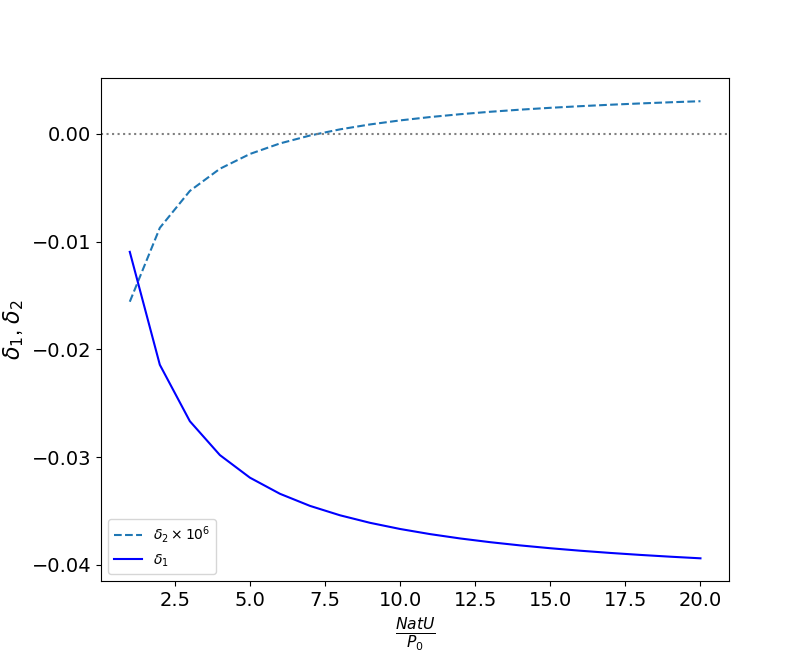
\includegraphics[width=.8\linewidth]{images/plots/7}  
    \caption{Концентрация $^{235}$U в предварительно обогащенном регенерата равна 7\%}
    \label{delta1}
  \end{minipage}
  \begin{minipage}{.5\textwidth}
    \centering
    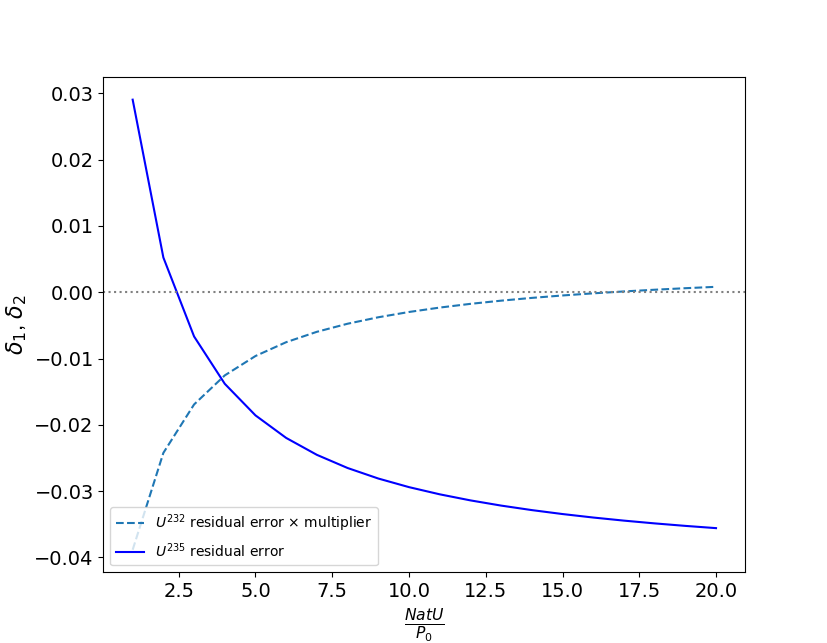
\includegraphics[width=.8\linewidth]{images/plots/15}  
    \caption{Концентрация $^{235}$U в предварительно обогащенном регенерата равна 15\%}
    \label{delta2}
  \end{minipage}
  \begin{minipage}{.5\textwidth}
    \centering
    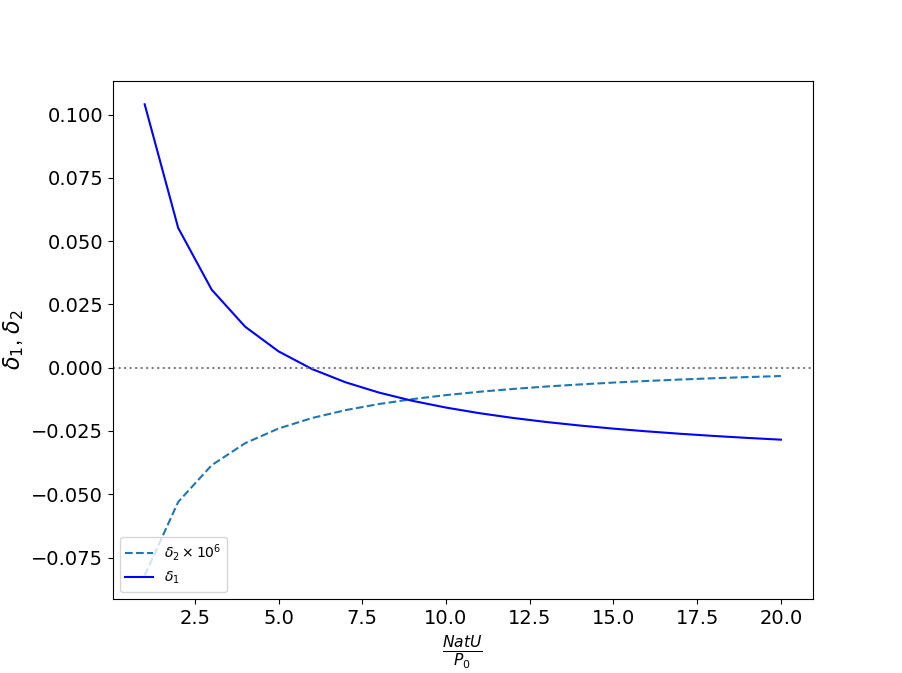
\includegraphics[width=.8\linewidth]{images/plots/30}  
    \caption{Концентрация $^{235}$U в предварительно обогащенном регенерата равна 30\%}
    \label{delta3}
  \end{minipage}
  \begin{minipage}{.5\textwidth}
    \centering
    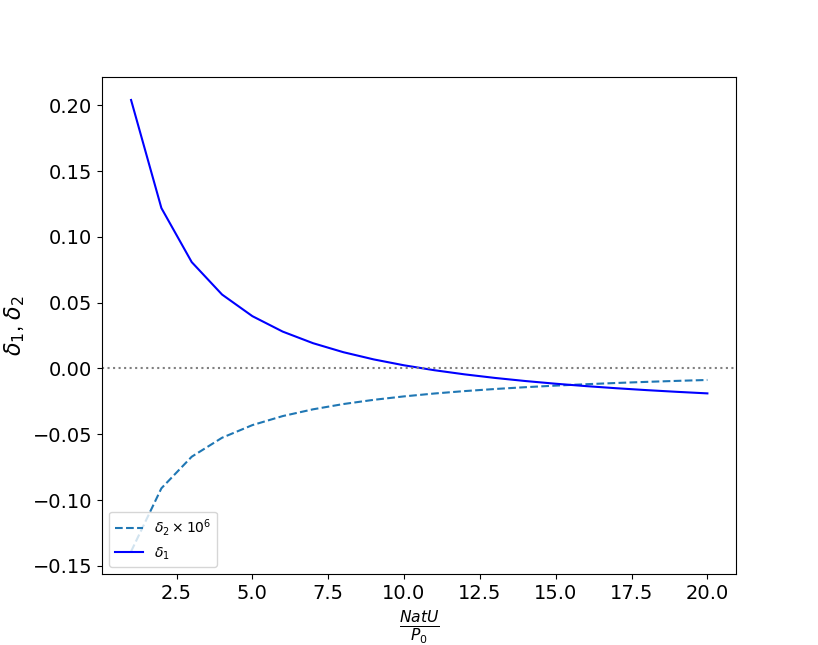
\includegraphics[width=.8\linewidth]{images/plots/50}  
    \caption{Концентрация $^{235}$U в предварительно обогащенном регенерата равна 50\%}
    \label{delta4}
  \end{minipage}
 \end{figure}

Как видно из рисунков \ref{delta1}-\ref{delta4} функции $\chi_1$ во всех случаях оказывается равной 0 в случаях, когда $\chi_2$ оказывается отрицательной, что означает превышение предельно допустимого значения концентрации $^{232}$U в продукте. Таким образом, полученные результаты показывают невозможность одновременного удовлетворения условия компенсации $^{236}$U и выполнения заданного ограничения по $^{232}$U в получаемом товарном НОУ. Очевидно, что в случае обогащения регенерата состава №2 ситуация окажется ещё более худшей, ввиду более высокого исходного содержания четных изотопов. 

Полученные результаты свидетельствуют о том, что данную схему нельзя рассматривать в качестве способа обогащения регенерированного урана в условиях его многократного рецикла, по крайней мере для выбранных в данном примере или более строгих ограничениях на концентрацию $^{232}$U. Основная причина таких результатов состоит в том, что рассматриваемая схема имеет количество свободных параметров, меньшее, чем количество условий требующих одновременного выполнения. Поэтому только в частных случаях возможно решить задачу, например, когда в обогащение поступает регенерированный уран с относительно низким исходным содержанием четных изотопов, что может соответствовать, например, обогащению регенерата первого рецикла.


\subsection{Схема с разбавлением предварительно обогащенного регенерата низкообогащенным ураном}\label{ch2_1_1}

Если в схеме, рассмотренной выше (рис. \ref{o1}), заменить разбавитель $(F_n)$ с природного урана на низкообогащенный уран, не содержащий четных изотопов (например, изготовленный из природного урана), то у подобной схемы, тем самым, появится дополнительный управляющий параметр -- концентрация $^{235}$U в потоке $F_n$, которую можно также варьировать.  Несмотря на это, в подобном варианте каскадной схемы все еще может быть не выполнено условие максимального использования регенерированного урана, состоящее в равенстве отношения потоков $E$ и $P$ заданной величине, так как количество свободных параметров все равно будет меньшим, чем количество условий. В качестве еще одного параметра схемы можно рассматривать концентрацию $^{235}$U в потоке отвала каскада -- $C_{235, W}$. Необходимо учесть, что данную величину возможно варьировать только в относительно узком диапазоне от 0,1\% до 0,6\% или ниже. 

Для оценки возможности решения задачи с использованием каскадной схемы рисунка \ref{o1} проведены вычислительные эксперименты, в рамках которых варьировались следующие параметры схемы:
\begin{enumerate}
  \item концентрация $^{235}$U в потоке $P_0$ ($C_{235, P_0}$);
  \item концентрация $^{235}$U в потоке $F_n$ ($C_{235, F_n}$);
  \item концентрация $^{235}$U в потоке $W$ ($C_{235, W}$).
\end{enumerate}

Варьирование этих параметров позволяет регулировать относительные концентрации компонентов в смеси, в частности, пары изотопов $^{232}$U и $^{235}$U. Это позволяет обеспечивать получение различных вариантов изотопного состава конечного продукта, возможно один из которых сможет удовлетворить все заданные ограничения одновременно. 

В части основных параметров каскада расчеты проводили при тех же значениях, что и в примерах, описанных в разделе \ref{ch2_1_1}. Как показали результаты расчетов, рассматриваемая модификация каскадной схемы обогащения регенерата позволяет одновременно удовлетворить все ограничения на концентрации четных изотопов в продукте. Однако ни в одном из рассчитанных вариантов не удалось добиться получения заданного отношения между исходным регенератом и продуктом. Данное утверждение иллюстрирует рисунок \ref{Figure_10}. Анализ кривых на указанном рисунке показывает невозможность выполнить условия возврата заданной доли регенерата на единицу продукта в такой каскадной схеме в доступном диапазоне варьирования её свободных параметров. Причем отношение используемого регенерата к НОУ-продукту меняется лишь незначительно с изменением $C_{235, W}$, и остается постоянным при разных концентрациях $C_{235, P_0}$. Последнее означает, что изменение данного параметра может оказывать влияние на величину затрат работы разделения или расхода природного урана, но не на долю возвращаемого в воспроизводство топлива регенерата.

\begin{figure}[ht]
  \centerfloat{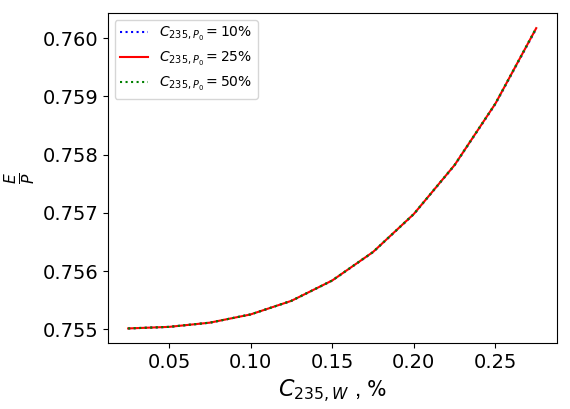
\includegraphics[scale=0.5]{images/plots/3_6}}
  \caption{Расход регенерата на единицу конечного НОУ-продукта для различных  $C_{235, P}$ и $C_{235, W}$ каскада, обогащающего регенерат (кривые совпадают)}\label{Figure_10}
\end{figure}

% , для которого удельный расход природного урана составляет $\approx$7,93 (см. Приложение).

% \begin{figure}[ht]
%   \centerfloat{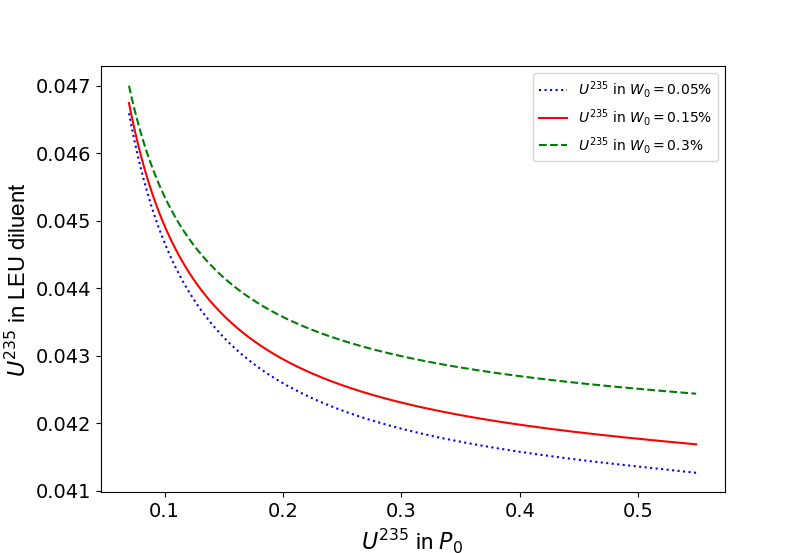
\includegraphics[scale=0.5]{images/plots/sc2_LEU_D}}
%   \caption{Концентрация $^{235}$U в разбавителе, необходимая для получения свежего НОУ для различных концентраций $^{235}$U в потоках продукта и отвала каскада, обогащающего регенерат}\label{fig:sc2_LEU_D}
% \end{figure}

% Проиллюстрировать затраты на работу разделения от составных  частей каскадной схемы, можно с помощью рис.\ref{myplot}, который показывает, что доля центрифуг для приготовления разбавителя из природного урана выше, чем доля центрифуг, задействованных для предварительного обогащения регенерата, и эта пропорция уменьшается с понижением содержания $^{235}$U в $W_0$.

% \begin{figure}[ht]
%   \centerfloat{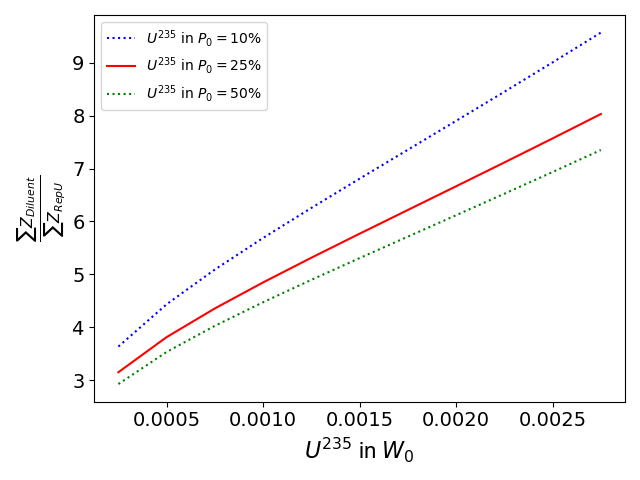
\includegraphics[scale=0.5]{images/plots/myplot}}
%   \caption{Отношение количества центрифуг в каскаде, производящем разбавитель из природного урана, к количеству центрифуг, задействованных для предварительного обогащения регенерата, для различных концентраций $^{235}$U в потоках продукта и отвала каскада, обогащающего регенерат}\label{myplot}
% \end{figure}

Рисунок \ref{fig3__7} иллюстрирует изменение концентрации $^{235}$U в разбавителе $(F_n)$ для различных концентраций этого же изотопа в потоках $P_0$ и $W$. Для каждой из точки на графиков удалось выполнить все ограничения на концентрации четных изотопов в товарном НОУ. Как видно, несмотря на возможность варьирования концентрации $^{235}$U в разбавителе, допустимый диапазон оказывается фактически узким (от 4,1 до 4,6\%). Данное обстоятельство можно объяснить тем, что фактически при смешивании разбавителя и обогащенного регенерата основная доля по массе приходится на разбавитель. Это означает, что концентрация в нем не может заметно отличаться от требуемой концентрации $^{235}$U в конечном продукте.   

\begin{figure}[ht]
  \centerfloat{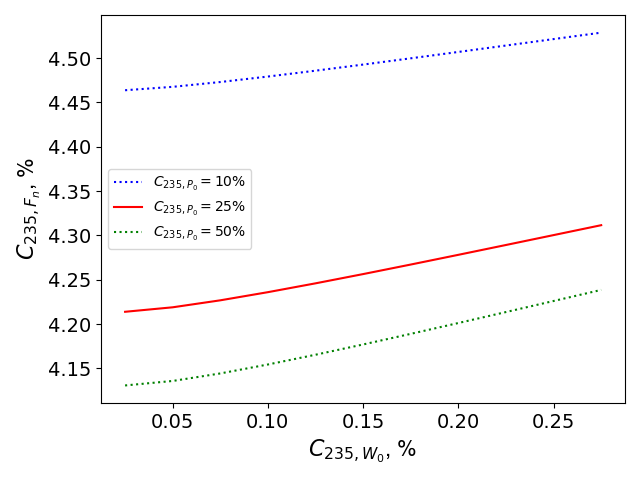
\includegraphics[scale=0.5]{images/plots/3__7}}
  \caption{Концентрация $^{235}$U в НОУ-разбавителе $F_n$ для различных $C_{235, P}$ и $C_{235, W}$ каскада, обогащающего регенерат}\label{fig3__7}
\end{figure}

Подытоживая анализ результатов вычислительных экспериментов для данной модификации ординарного каскада для обогащения регенерированного урана, можно заключить, что она непригодна для решения задачи обогащения в условиях многократного рецикла, так как с помощью нее нет возможности использовать весь регенерированный уран на производство НОУ-продукта, как показано на рис. \ref{Figure_10}. Тем не менее, рассмотренная каскадная схема может быть использована для решения задачи повторного использования урана для возврата (дообогащения) регенерата с относительно низким исходным содержанием чётных изотопов, что соответствует первому рециклу или низкой глубине выгорания топлива.

\subsection{Анализ схемы с разбавлением предварительно обогащенного природного урана регенератом}

Проанализируем возможность решения задачи обогащения регенерированного урана со всеми ограничениями в каскадной схеме с разбавлением предварительно обогащенного природного урана регенератом (рис. \ref{o2}). Принцип работы такой схемы состоит в том, что предварительно обогащенный природный уран смешивается с возвращаемым в топливный цикл регенерированным ураном. Уровень предварительного обогащения (перед смешением) природного урана и отношение потоков обогащенного природного урана к регенерату определяются исходя из условий задачи. Таким образом, данная схема в принципе аналогична схеме рисунка \ref{o1}. Это означает, что ей присущ тот же принципиальный недостаток, что и упомянутой схеме, а именно: число ее управляющих параметров меньше, чем число условий, требующих одновременного выполнения. 

\begin{figure}[ht]
  \centerfloat{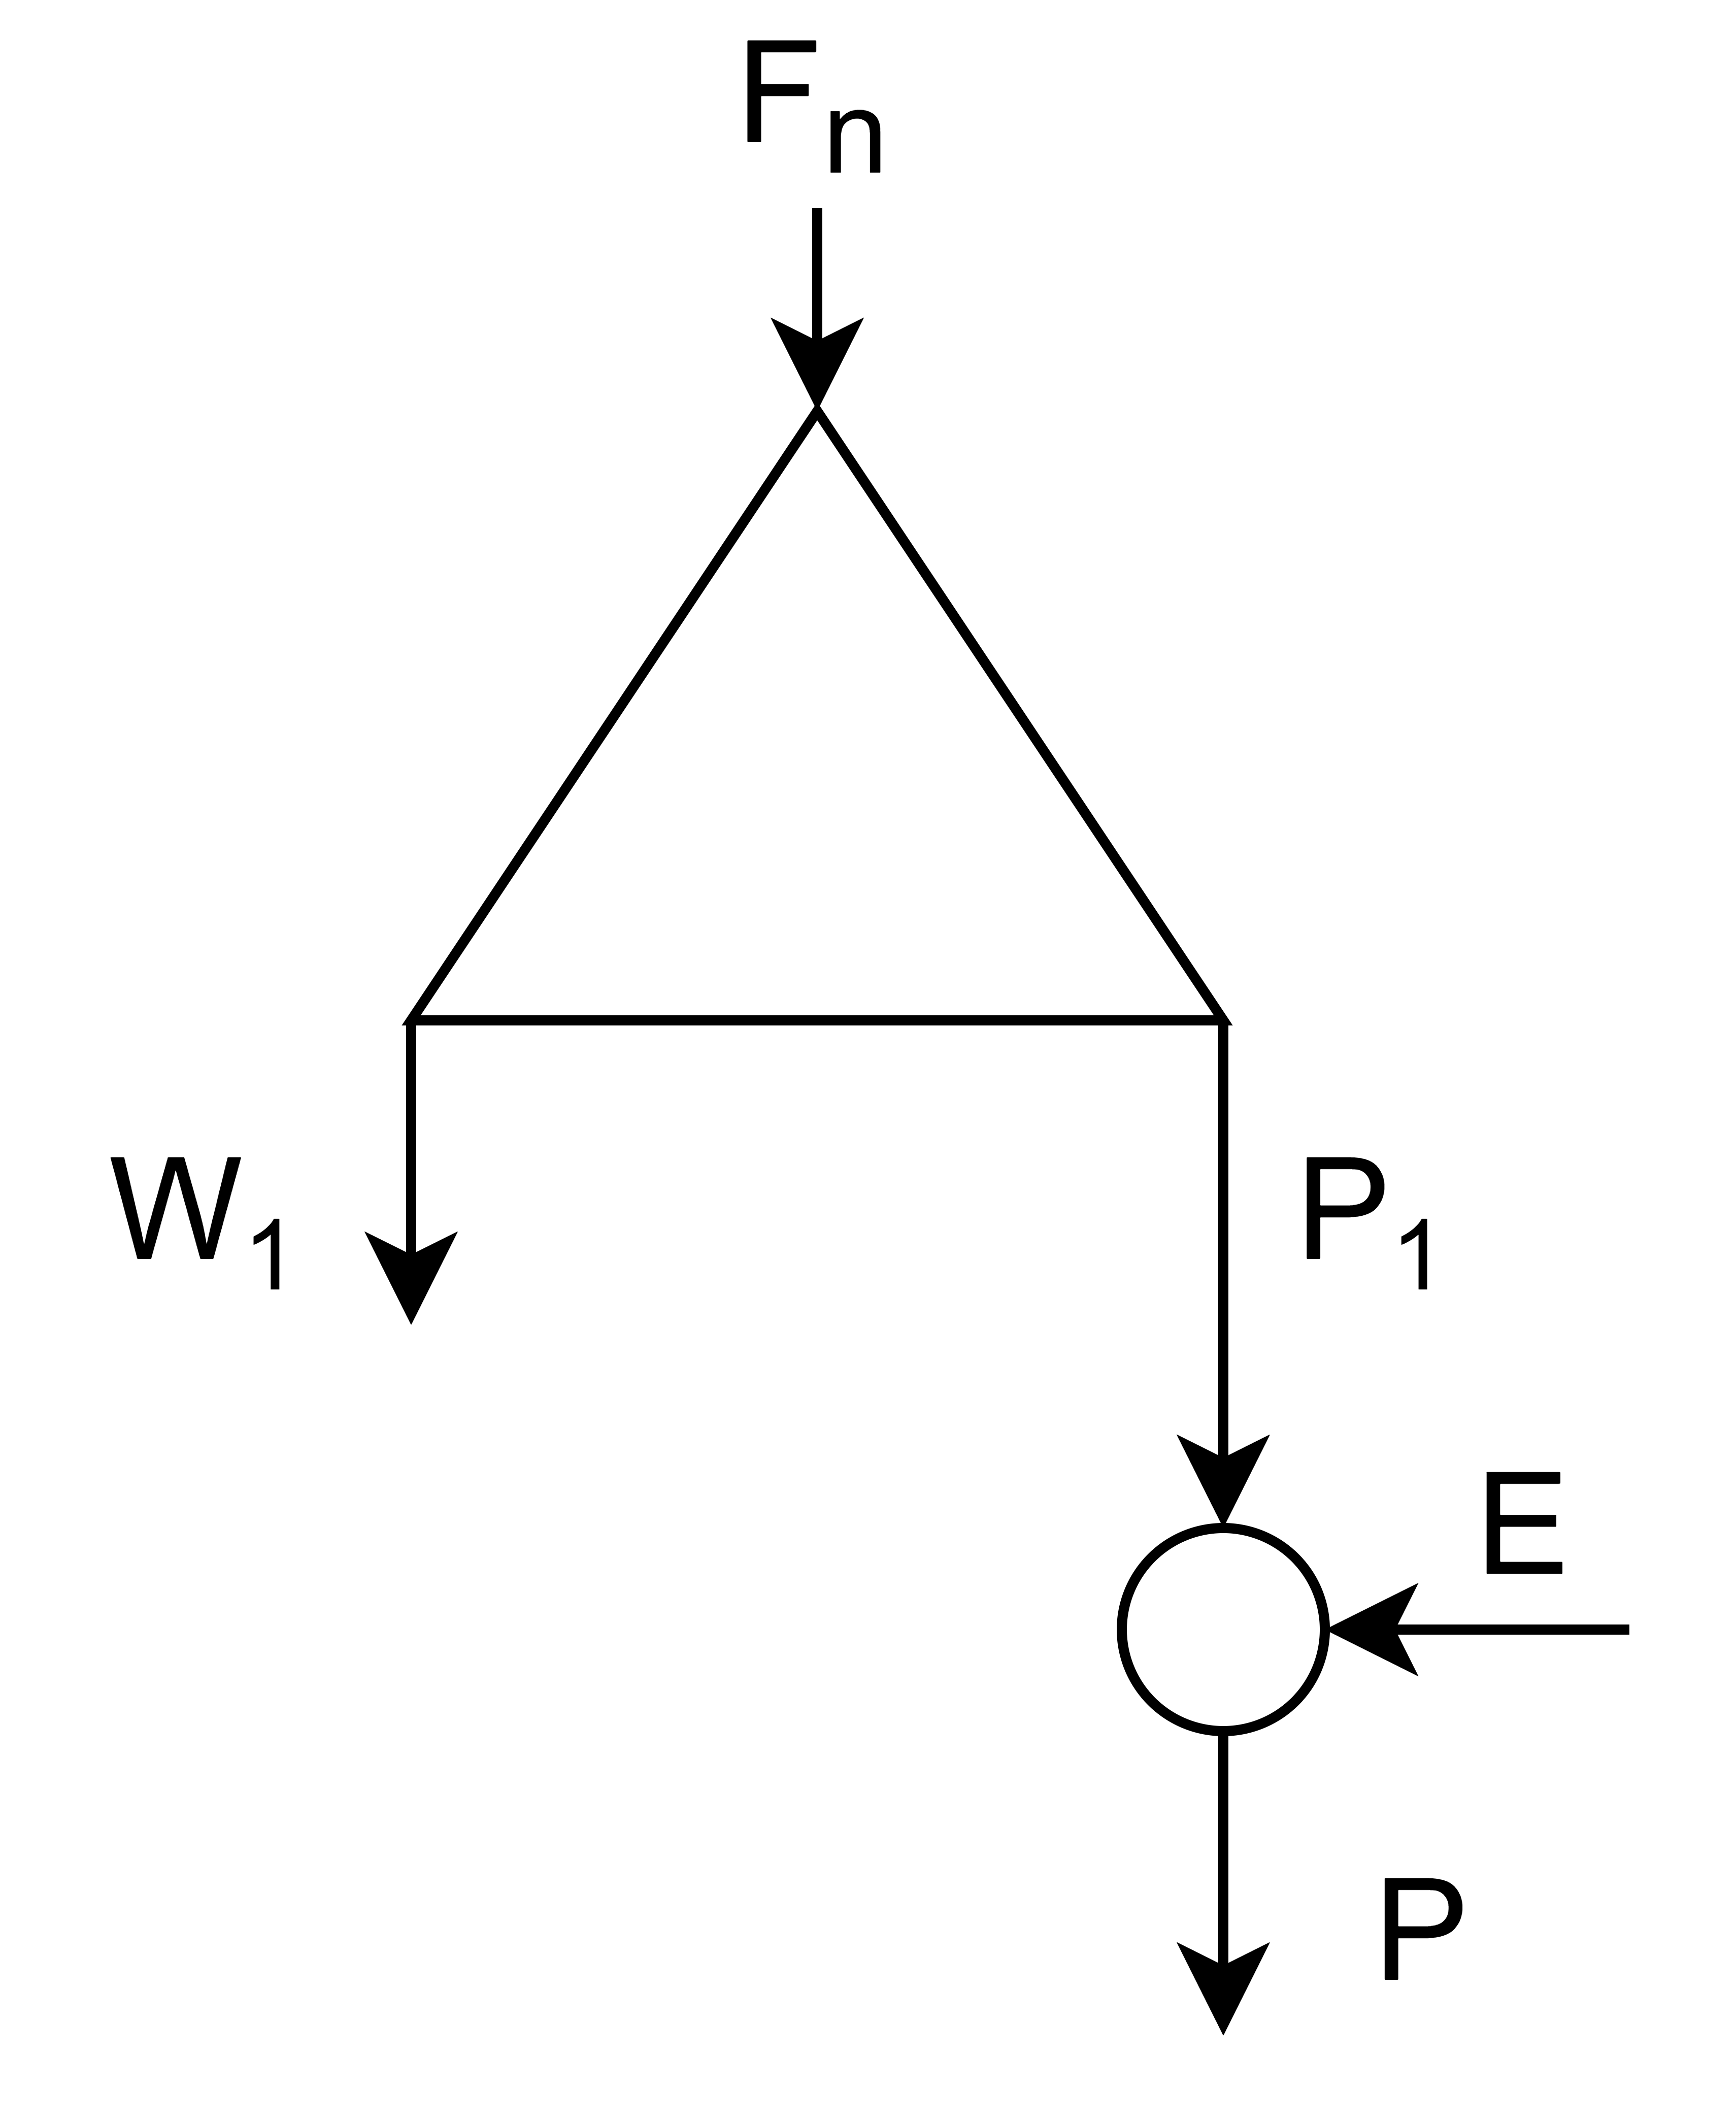
\includegraphics[scale=1.1]{cascades/ord2}}
  \caption{Схема каскада с разбавлением предварительно обогащенного природного урана регенератом. Обозначения: $E$ -- регенерат, $F_n$ -- природный уран; $W$ -- поток отвального ОГФУ тяжелого конца каскада; $P$ -- поток товарного низкообогащенного урана}\label{o2}
\end{figure}

Для ответа на вопрос о возможности использования данной схемы для обогащения регенерата в условиях многократного рецикла были проведены вычислительные эксперименты, в рамках которых варьировали величину концентрации $^{235}$U в обогащенном природном уране и отношение, в котором смешиваются разбавитель с регенератом с целью найти такой набор параметров схемы, при которых сформулированная в разделе \ref{ch2_stat} задача будет решена. Как и в рассмотренных выше примерах моделирование процесса обогащения урана в каскаде осуществляли с использованием $R$-каскада. Концентрацию $^{235}$U в отвале каскада задавали равной 0,1\%.

Из результатов вычислительных экспериментов следует, что для рассматриваемой схемы возможно получение решения, удовлетворяющего заданным ограничениям на концентрации изотопов $^{232,234,236}$U. Однако, как и в случае применения схемы рис. \ref{o1}, одновременно с этими условиями не удаётся удовлетворить условие возврата заданной массы регенерата. В результате вместо заданной величины отношения массы исходного регенерата к продукту -- 0,93, фактические значения не превысили величины 0,755. Данные результаты свидетельствуют о том, что такая схема обогащения регенерата не решает поставленную задачу для произвольного изотопного состава регенерата и, следовательно, не может быть применена в условиях многократного рецикла урана в топливе легководных реакторов.

\subsection{Анализ схемы с разбавлением регенерата природным ураном перед подачей в ординарный трехпоточный каскад}

Еще одним вариантом каскадной схемы для обогащения регенерированного урана, основанной на использовании ординарного каскада является схема, в которой смешивание и разбавление регенерата происходит непосредственно перед подачей в каскад для последующего обогащения (рис. \ref{o3}). В качестве разбавителя здесь, как правило, рассматривают природный уран. Соотношение, в котором следует смешать природный и регенерированный уран определяют, исходя из ограничений на концентрации четных изотопов в конечном НОУ-продукте.

\begin{figure}[ht]
  \centerfloat{
\includegraphics[scale=1.1]{cascades/ord3}}
  \caption{Схема каскада со смешением регенерата и природного урана перед подачей на питание ординарного каскада. Обозначения: $E$ -- поток питающего схему регенерата, $F_n$ -- поток разбавителя; $W$ -- поток отвального ОГФУ тяжелого конца каскада; $P$ -- поток товарного низкообогащенного урана}\label{o3}
\end{figure}

В случае, если разбавитель известен, то для такой схемы существует единственный управляющий параметр -- это отношение, в котором смешиваются потоки регенерата и природного урана. Очевидно, что с ростом доли регенерата в совокупном питании каскада (смесь потоков $E$ и $F_n$) будут возрастать концентрации чётных изотопов в потоке отбора каскада. Это обуславливает тот факт, что существует некоторое критическое значение этого отношения, начиная с которого уже невозможно будет соблюсти, как минимум, ограничение на концентрацию изотопа $^{232}$U. Для рассматриваемой схемы проведены вычислительные эксперименты, в которых варьировали отношение разбавления между регенератом и разбавителем, в качестве которого рассматривали уран природного состава. Кроме того, в диапазоне 0,05--0,3\% варьировали концентрацию изотопа $^{235}$U в потоке отвала каскада -- $C_{235, W}$. Как и во всех рассмотренных в рамках данной главы примерах исходные условия соответствовали задаче, описанной в разделе \ref{ch2_stat}, а в качестве расчётной модели использован $R$-каскад. Расчёты проведены на примере состава 1 таблицы \ref{is_compositions_2_5}. 

На рис. \ref{sc3_1.second} отражена взаимозависимость отношения потоков $E/P$ и концентрации $^{232}$U в конечном продукте. Кривые построены при различных $C_{235, W}$. Как следует из анализа представленных зависимостей, во всех случаях величина концентрации  $^{232}$U достигает предельного значения ($5\cdot10^{-7}$\%) ранее, чем отношение между исходным регенератом и продуктом достигнет требуемого значения -- 0,93. Это означает, что и эта схема также не позволяет решить полностью задачу обогащения регенерата с относительно высоким содержанием чётных изотопов, не позволяя расходовать заданное количество регенерата на единицу конечного НОУ-продукта. Иными словами схема также оказывается непригодной к обогащению регенерированного урана в условиях многократного рецикла в допустимом диапазоне изменения ее параметров.

\begin{figure}[ht]
  \centerfloat{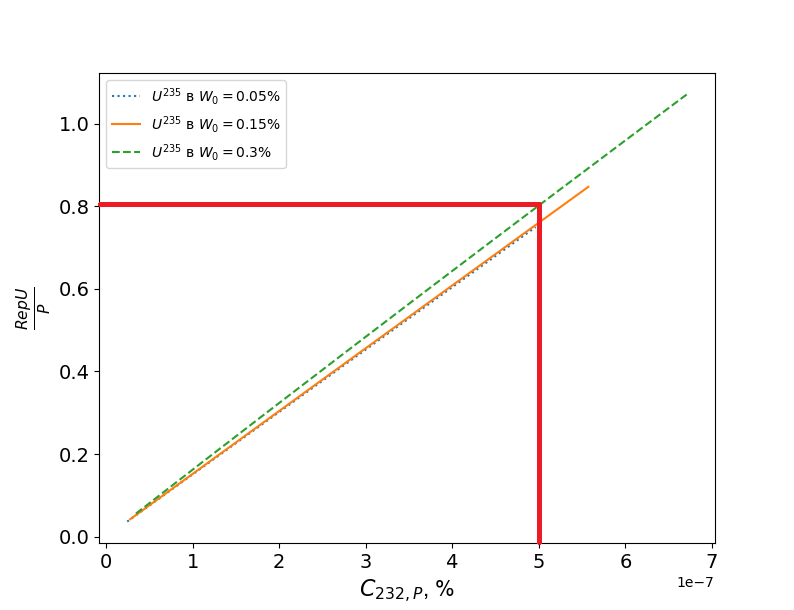
\includegraphics[scale=0.5]{images/plots/3_11}}
  \caption{Расход регенерированного урана на единицу НОУ-продукта  при различной концентрации $^{232}$U в питающем потоке каскада для различных концентраций $^{232}$U в потоке НОУ-продукта}\label{sc3_1.second}
\end{figure}


% \begin{figure}[ht]
%   \centerfloat{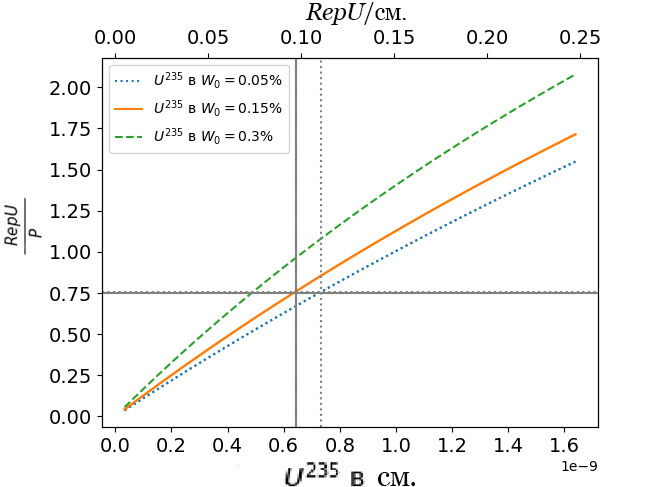
\includegraphics[scale=0.5]{images/plots/3.11new}}
%   \caption{Расход регенерированного урана на единицу НОУ-продукта  при различной концентрации $^{232}$U в питающем потоке каскада для различных концентраций $^{235}$U в потоке отвала. Обозначения: см. - смесь природного урана и регенерата, подаваемая на питание каскада}\label{sc3_1.second}
% \end{figure}

\subsection{Аналитический подход к оценке возможности использования модификаций ординарного каскада для обогащения регенерированного урана в условиях многократного рецикла}

Описанные выше результаты вычислительных экспериментов, проведенных для оценки применимости схем на основе ординарного каскада для решения задачи обогащения регенерированного урана, показали что такие схемы не могут решить подобную задачу в условиях  многократного рецикла. Это обусловлено ухудшением изотопного состава урана по мере прохождения им серии топливных циклов, что выражается в накоплении $^{232}$U и других чётных изотопов. При этом исходная концентрация $^{232}$U питающей смеси, начиная со второго рецикла, превышает уровень допустимый в конечном продукте, поэтому схемы, основанные на ординарном каскаде, которые только разбавляют этот изотоп, не эффективны для решения поставленной задачи. Тем не менее, если рассматривать подобные схемы для обогащения регенерированного урана, прошедшего только однократное облучение или допустить <<послабление>> ограничений на концентрации чётных изотопов, то подобные схемы, безусловно, могут быть применены для решения задачи обогащения регенерированного урана.

При этом закономерно возникает следующий вопрос: возможно ли априорно оценить возможность решить поставленную в (\ref{ch2_stat}) задачу в таких модификациях ординарного каскада? 

На этот вопрос можно ответить, обратившись к уравнениям баланса компонентов в каскаде (\ref{GrindEQ__1_21_}) по крайней мере в случае вариантов каскадных схем, где регенерированный уран поступает в каскад для обогащения. Запишем уравнение (\ref{GrindEQ__1_21_}) для изотопа $^{232}$U и, учитывая, его малую концентрации в исходной смеси, сделаем предположение о том, что его концентрация в отвале каскада будет стремиться к нулю. Данное предположение может быть вполне оправдано, если отвальная часть каскада имеет достаточное число ступеней. В этом случае $^{232}$U, являясь самым лёгким в смеси регенерированного урана, будет активнее остальных компонентов концентрироваться в отборе каскада. Это означает, что для изотопа $^{232}$U уравнение (\ref{GrindEQ__1_21_}) можно переписать в следующем виде, пренебрегая слагаемым с потоком отвала каскада:

\begin{equation} \label{GrindEQ__1_21__} 
  \begin{array}{l} {\quad \quad \quad \quad \quad  E+F=P+W,} \\ {FC_{i,F} + EC_{i,E} =PC_{i,P} +WC_{i,W} ,\;  i=1,2,...,m.} \end{array} 
\end{equation} 

% \begin{equation}
% \label{eq_232_balance}
%   C_{232,P} \approx \frac{RepU}{P} C_{232,RepU}
% \end{equation}

\begin{equation}
  \label{eq_232_balance_}
    C_{232,P} \approx \frac{E}{P} C_{232,E}
  \end{equation}

Величина $\frac{E}{P}$ в приведенном выше уравнении и является отношением (исходный регенерат)/продукт. Если учесть, что типичные значения этого отношения составляют величину $\approx$0,9-0,95, то станет очевидно, что это условие будет выполнено только, если концентрация $^{232}$U в исходном регенерате ниже, чем ограничение на $^{232}$U в конечном продукте. 
С помощью уравнения (\ref{eq_232_balance_}) можно вычислить максимально возможную долю питающего потока, содержащего $^{232}$U, как неизвестную переменную уравнения (\ref{eq_232_balance_}). Например, для состава 1 таблицы \ref{is_compositions_2_5}, который был использован в рассмотренных выше примерах получаем:

% \begin{equation}
%   \label{eq_232_balance_X}
%     5 \times 10^{-7} \% \approx X \times 6.622 \times 10^{-7} \% \Rightarrow X \approx 0.755
% \end{equation}

% \begin{equation}
%   \label{eq_232_balance_X}
%     \frac{RepU}{P} \leq 0,755
% \end{equation}

\begin{equation}
  \label{eq_232_balance_X_}
    \frac{E}{P} \leq 0,755
\end{equation}

% \begin{equation}
%   \label{eq_232_balance_X_}
%     \frac{E}{P} \leq 0,5
% \end{equation}

Снова анализируя представленные в предыдущих разделах данные, легко увидеть, что полученные в результате прямого численного расчёта предельные величины отношений (исходный регенерат)/продукт приблизительно и составляют такую величину.

\textcolor{red}{Важно сделать акцент на том, что в случае $\frac{E}{P}\leq 0,755$ вместо требуемых в рассматриваемом примере $\frac{E}{P}=0,93$, в процессе возврата урана в топливный цикл ещё до начала его обогащения происходит потеря 17,5\% $^{235}$U, который остается незадействован в воспроизводстве НОУ. Причем эта потеря предшествует потерям, которые далее неминуемо возникают при обогащении в связи с уходом части целевого изотопа в поток отвала каскада. Это означает, что фактические потери целевого изотопа $^{235}$U в таком каскаде будут ещё больше и по оценкам могут достигать 25-30\% от исходной массы $^{235}$U в поступившей в обогащение массе регенетата.}

Используя уравнение (\ref{eq_232_balance_}), легко оценить максимальное содержание $^{232}$U в исходном регенерате, при котором еще будет возможно решить задачу обогащения регенерата. Это можно сделать, подставив в (\ref{eq_232_balance_}) величины $C_{232,P}$ и $\frac{E}{P}$ и вычислив $C_{232,E}$. Например, для $\frac{E}{P}=0,93$ и $C_{232,P}=5\cdot10^{-7}\%$ получаем величину $\approx 5,37\cdot10^{-7}\%$, что оказывается меньше, чем в составах №1 и №2 таблицы \ref{is_compositions_2_5}.

Описанный выше подход позволяет аналитически оценить возможность применения схем на основе простейших модификаций ординарного каскада, исходя из изотопного состава регенерата. Следует отметить, что подобные оценки можно также применять и для каскадных схем, в которых регенерат разбавляют уже внутри каскада, путём его подачи в качестве дополнительного питания, поскольку такие схемы по сути являются также только разбавляющими, а балансные соотношения для них будут выглядеть аналогично (\ref{GrindEQ__1_21__}).

\subsection{Общий вывод для схем возврата регенерата в ЯТЦ на основе ординарного каскада}\label{sec:ch2/sec2}

Обобщая описанные выше результаты вычислительных экспериментов, проведенных для различных модификаций ординарного каскада для обогащения и разбавления регенерированного урана, можно сделать следующие основные выводы:
\begin{enumerate}
  \item Представленные на рисунке \ref{fig:diagram1ch3} варианты каскадных схем принципиально не решают задачу обогащения регенерированного урана при одновременном выполнении условий на концентрации четных изотопов в товарном НОУ и обеспечения расходования заданной массы регенерата на получение этого НОУ для составов регенерата с исходным высоким содержанием четных изотопов. Например, для концентраций $^{232}$U, исходно превышающих предельные значения для товарного НОУ. 
  \item Основная причина невозможности решения задачи состоит в том, что в рассматриваемых схемах число свободных параметров оказывается меньшим, чем число условий, которые необходимо одновременно удовлетворить. В результате такие схемы могут обеспечить решение задачи только в некоторых частных случаях, например, когда в обогащение поступает регенерированный уран с относительно низкими исходными концентрациями четных изотопов, что может соответствовать обогащению регенерата первого рецикла.
  \item Продемонстрирован аналитический подход к оценке возможности применения схем на основе ординарного каскада для решения задачи, основанный на анализе исходного изотопного состава поступающего в обогащение регенерированного урана.
  \item Полученные результаты однозначно свидетельствует о том, что для обогащения регенерированного урана в условиях многократного рецикла необходимо использование более сложных вариантов каскадных схем, которые смогут позволить полностью решить поставленную задачу обогащения регенерата безотносительно к его исходному составу и другим внешним условиям.
\end{enumerate}

\section{Обоснование необходимости составных схем}\label{sec:ch2/sec2}

Как следует из описанных выше результатов, на текущий момент в принципе имеются способы, позволяющие обеспечить выполнение требований по четным изотопам урана при обогащении регенерата. Однако основной проблемой, решаемой в рамках настоящей диссертационной работы, является поиск варианта каскадной схемы, позволяющей одновременно выполнить ограничения по концентрациям четных изотопов и задействовать в обогащении весь имеющийся регенерат в условиях неопределенности его изотопного состава при многократном рецикле.

Если анализировать причины невозможности возврата массы регенерата в производство топлива в различных модификациях ординарного каскада для обогащения регенерата в условиях многократного рецикла, то становится очевидным, что это, во многом, связано с нарастанием относительных концентраций <<легких>> изотопов (в первую очередь $^{232}$U) и $^{235}$U. Поскольку данные изотопы концентрируются вместе на легком <<конце>> каскада, то единственным способом понизить отношение их концентраций -- это разбавить материалом, не содержащим $^{232}$U, $^{236}$U. Как показали результаты, описанных в этой главе вычислительных экспериментов, для составов с относительно высоким исходным содержанием $^{232}$U невозможно подобрать такой разбавитель, чтобы удовлетворить одновременно и условие полного возврата массы регенерата в цикл и ограничения на содержание четных изотопов.

Из приведенного выше анализа следует, что эффективная каскадная схема для обогащения регенерата урана при многократном рецикле должна обеспечивать не только разбавление регенерата, но и частично его очистку от чётных изотопов. Поэтому возможные варианты решения задачи, по-видимому, должны быть основаны на использовании схем двойных каскадов, в том числе, описанных в Главе \ref{ch1}. В связи с этим представляет интерес оценка возможности прямого обогащения регенерата с повышенным содержанием чётных изотопов в двойном каскаде с целью решения задачи обогащения регенерата в наиболее общей постановке. Этот вопрос и рассмотрен в следующих разделах настоящей главы.

\section{Двойной каскад}\label{sec:ch2/dvoynoy}

Двойной каскад для обогащения регенерата рассмотрен в литературном обзоре (см. \ref{ch1/dvoynoy}) и представляет собой последовательное соединение двух каскадов (рис. \ref{fig:double_ru_in3}). 

\begin{figure}[ht]
  \centerfloat{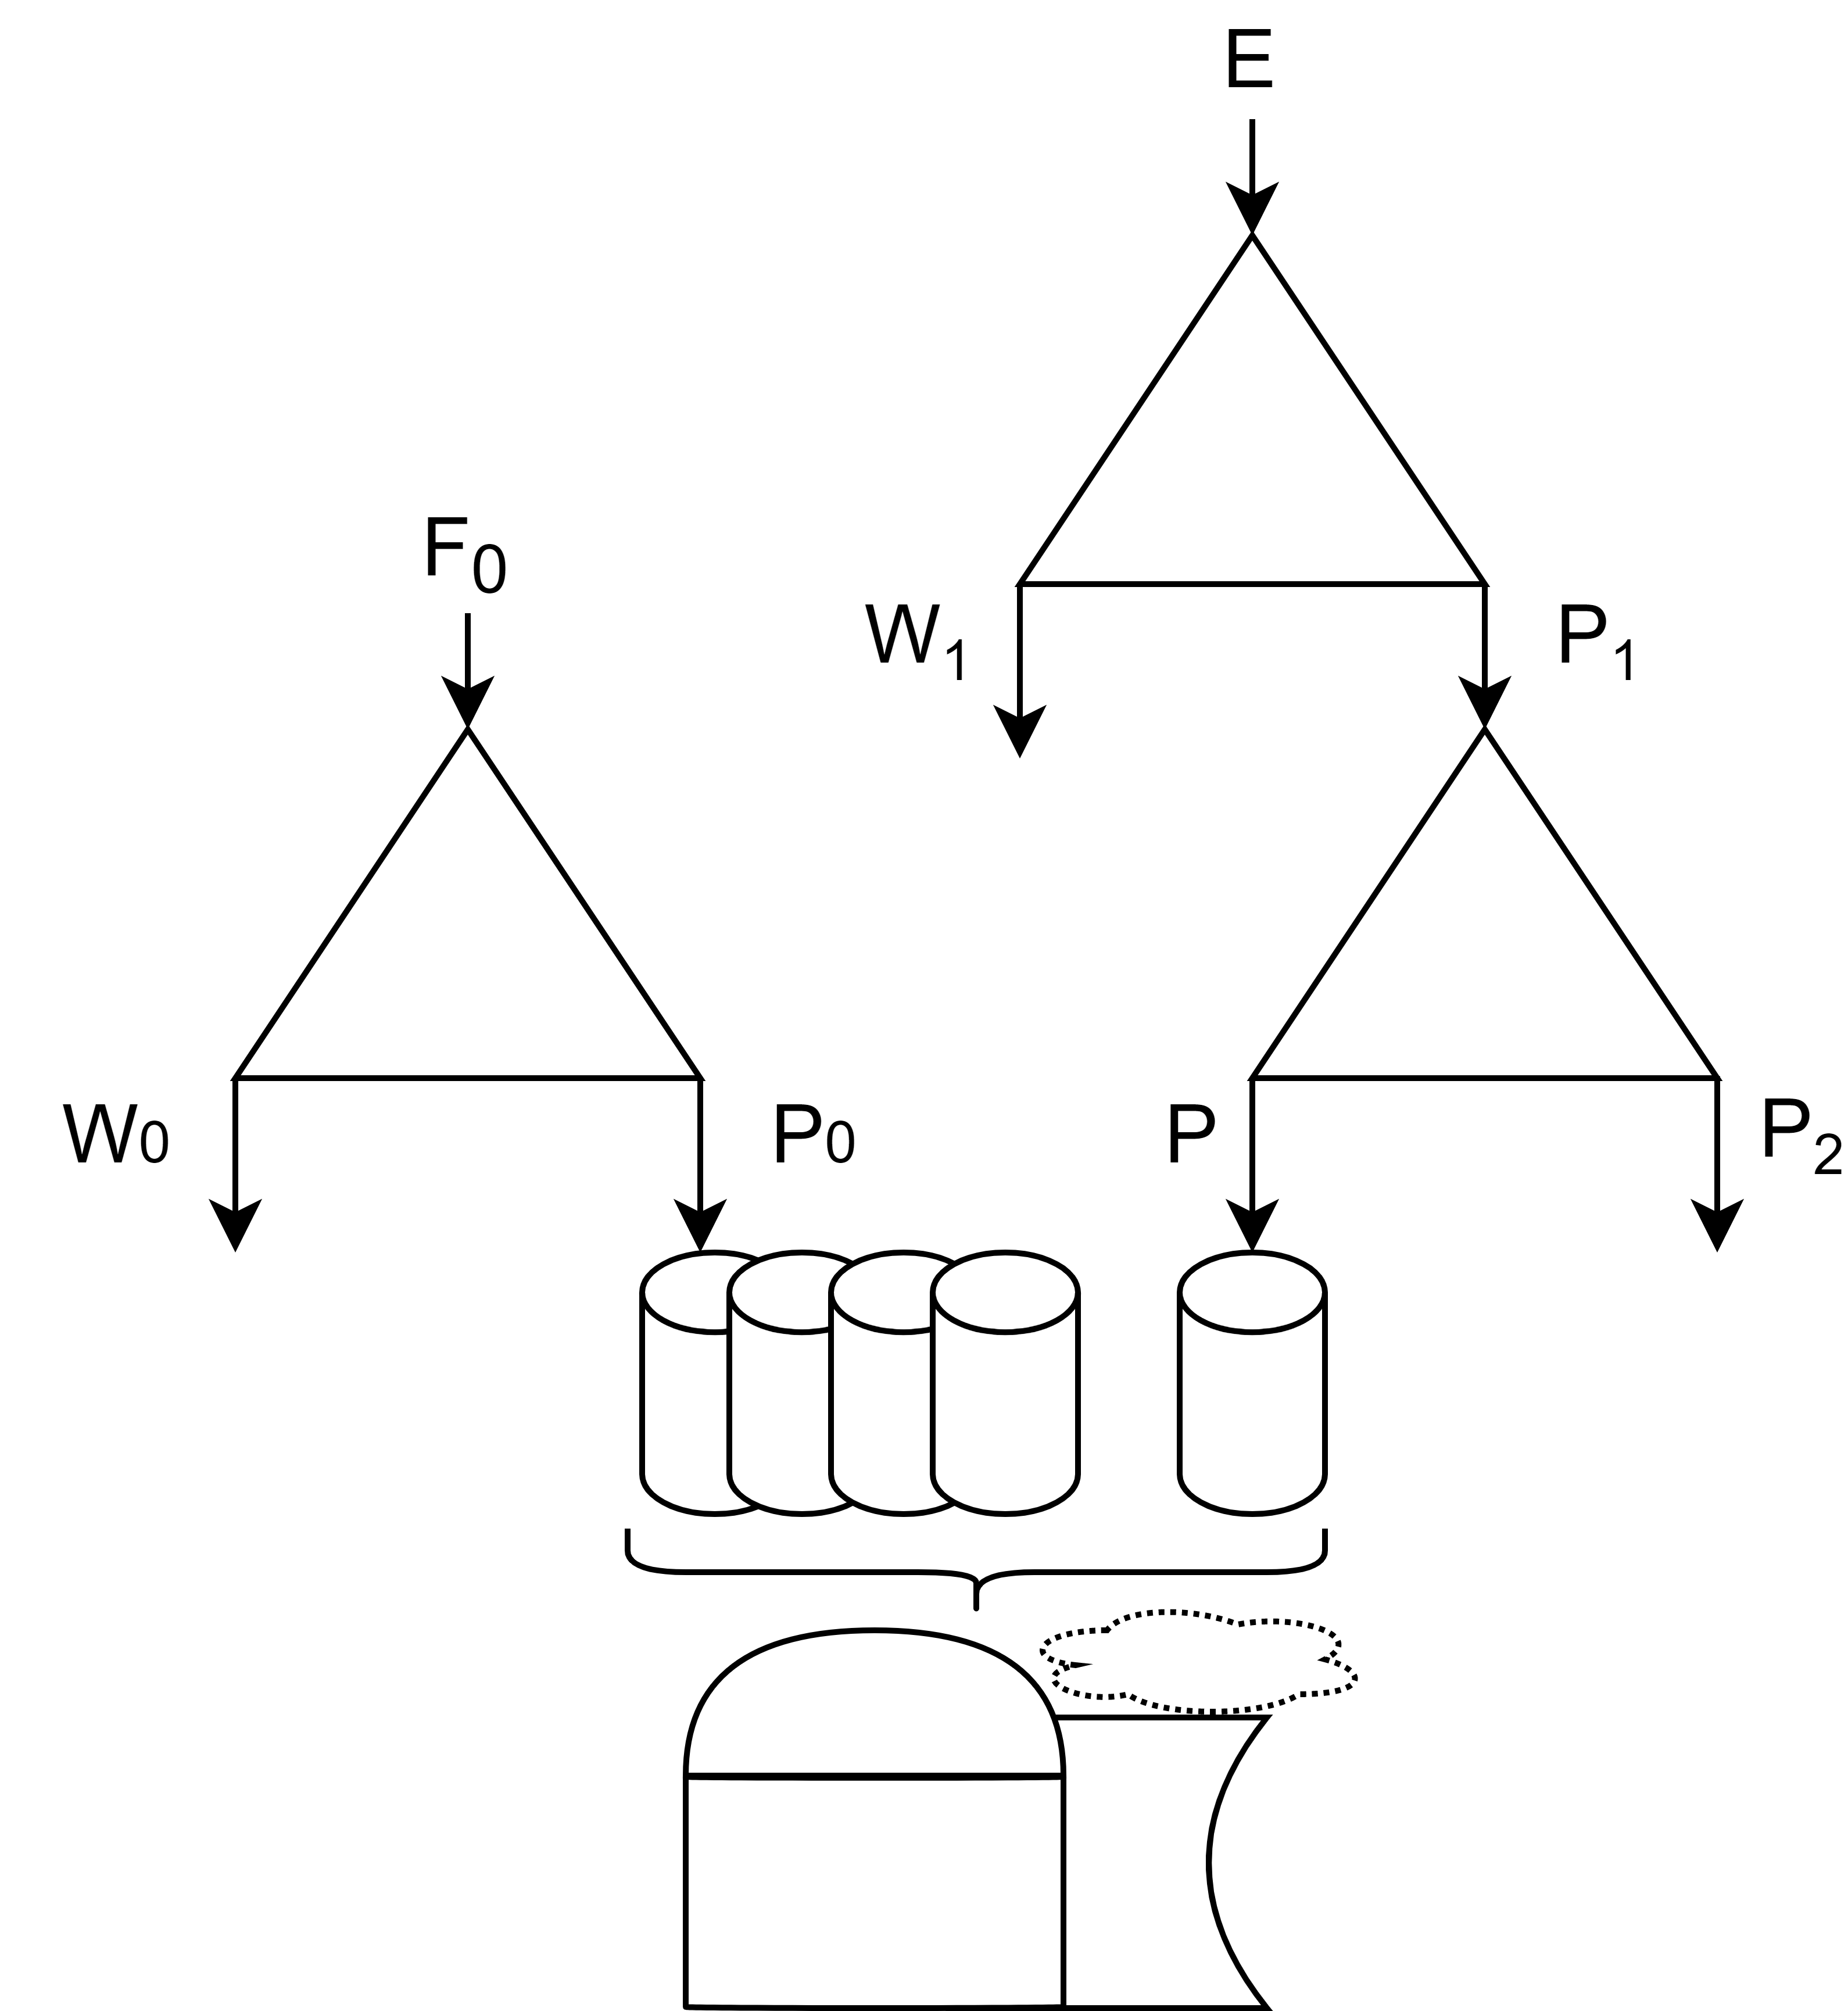
\includegraphics[scale=1.0]{cascades/Double_core}}
  \caption{Двойной каскад. Обозначения: $E$ -- поток питающего схему регенерата, $W_1$ -- поток отвального ОГФУ тяжелого конца каскада; $P$ -- конечный НОУ продукт на основе регенерата; $P_2$ -- отход двойного каскада в виде высокообогащенного урана; $F_0$ -- природный уран; $P_0$ -- дополнительно производимый НОУ продукт для возможности загрузить активную зону реактора}\label{fig:double_ru_in3}
\end{figure}

Напомним кратко суть работы этой схемы. Двойной каскад позволяет сконцентрировать нежелательные четные изотопы отдельно от изотопа $^{235}$U. Для этого сначала в каскаде I обогащают изотоп $^{235}$U с одновременным обогащением изотопов $^{232}$U, $^{234}$U, $^{236}$U, а затем полученную смесь направляют на вход каскада II (рис. \ref{fig:double_ru_in3}), где она делится на две группы: в первой обогащены легкие изотопы ($^{232}$U, $^{234}$U и $^{235}$U), во второй обедняется $^{235}$U с более интенсивным обеднением $^{232}$U, $^{234}$U. Это позволяет в потоке $W_2$ получить низкообогащенный уран, отвечающий требованиям по концентрациям изотопов $^{232}$U, $^{234}$U с одновременной компенсацией $^{236}$U.

Нужно учитывать, что для двойного каскада выполнено очевидное условие $E>W_2$, а чаще всего - $E \gg W_2$. Это означает, что при рассмотрении в рамках топливного цикла и необходимости обеспечения реактора ядерным топливом такой каскад может произвести лишь небольшую часть топлива для загрузки реактора. Остальную массу необходимо получить другим путём, например, обогащением природного урана. Это иллюстрирует третий каскад на рис. \ref{fig:double_ru_in3}, который нарабатывает недостающую массу ядерного топлива для загрузки реактора. В этом контексте интерес представляет оценка эффективности такой каскадной схемы в топливном цикле при условии обогащения регенерированного урана с относительно высоким содержанием чётных изотопов. Для этого в рамках работы проведены вычислительные эксперименты, направленные на получение ответа на эти вопросы. В качестве модели для описания процессов селективного массопереноса в каждом из каскадов схемы использован $R$-каскад. 

При этом рассматривали разделительную задачу в следующей постановке.

Задано:

\begin{itemize}
    \item концентрации компонентов в обогащаемом регенерированном уране -- $C_{i,{E}}$; 
    \item величина концентрации $^{235}$U в потоке $W_{1}$ -- $C_{235,{W_1}}$;
    \item параметры одиночного разделительного элемента (центрифуги) -- величины потока питания центрифуги ($l_{ГЦ}$) и коэффициента разделения, приходящегося на единичную разность массовых чисел ($q_{0}$);
    \item величина потока $E$ (определяется массой поступившего в обогащение регенерата);
    \item в случае использования $R$-каскада необходимо задание пары компонентов, по которым должно быть выполнено условие несмешивания их относительных концентраций (подробнее см. Главу \ref{ch2_theory}).
\end{itemize}

Параметры каскадной схемы должны соответствовать требованиям, предъявляемым к получаемому товарному НОУ:

\begin{itemize}
    \item величина концентрации $^{235}$U в продукте (товарном НОУ, поток $P$ ($P \equiv W_2$) на схеме рис. \ref{p2left}) -- $C_{235,{P}}$;
    \item величины предельных концентраций изотопов $^{232}$U и $^{234}$U в конечном продукте $P$ -- $(C_{232,{P}})_{lim}$;
    \item величины предельно допустимого отношения концентраций изотопа $^{234}$U и $^{235}$U в конечном продукте $P$ -- ${C_{234,{P}}}/{C_{235,{P}}}$;
    \item величина концентрации $^{235}$U в потоке отвала каскада I -- $C_{235,{W_1}}$;
    \item вид функции $f(C_{236,P})$, в соответствии с которой рассчитывают конечную (эквивалентную) величину обогащения по $^{235}$U в продукте, с учётом компенсации присутствия $^{236}$U:
    $(C_{235,P})_\textit{экв.}=(C_{235,P})_\textit{прир.}+f(C_{236,P})$.    
\end{itemize}

Расчёт параметров рассматриваемой каскадной схемы строится на основе результатов последовательного расчёта каждого из каскадов схемы. Причём для отдельных каскадов осуществляют проектировочный расчёт их параметров (см. Главу \ref{ch2_theory}), когда в качестве заданных величин выступают концентрации одного из компонентов смеси в потоках отбора и отвала каскада, а искомыми параметрами выступают полное число ступеней в каскаде и номер ступени подачи внешнего питания для R-каскада. Таким образом, для каждого из каскадов при заданных концентрациях компонентов в потоках питания, величине одного из внешних потоков ($F$, $P$ или $W$), параметрах одиночного разделительного элемента, для расчёта их остальных параметров необходимо задать ещё 2 величины. Такой парой параметров как раз и могут выступать концентрации целевого компонента в потоках отбора и отвала каскада. Задание этих величин позволяет, используя уравнения (\ref{GrindEQ__1_72_}), (\ref{GrindEQ__1_73_}), определить неизвестные величины $N$ и $f$ для каждого из каскада и далее по соотношениям (\ref{GrindEQ__1_70_})-(\ref{GrindEQ__1_77_}) рассчитать все их внешние и внутренние параметры. Тем самым имеем ситуацию, при которой для последовательного расчёта параметров каждого из каскадов схемы, учитывая, что величина $C_{235,{W_1}}$ задана по условию, необходимо задать ещё 3 величины: $C_{235,{P_1}}$, $C_{235,{P_2}}$ и $C_{235,{P}}\equivC_{235,{W_2}}$. Причём концентрация $C_{235,{P}}$ также попадает в эту группу, поскольку точное определение данной величины возможно только, если известна конечная концентрация $^{236}$U в НОУ, которую нужно скомпенсировать. Таким образом, неизвестными переменными задачи будут величины $C_{235,{P_1}}$, $C_{235,{P_2}}$ и $C_{235,{P}}$, определяющие полные числа ступеней и номера ступеней подачи питаний в каскадах I и II.    

Для нахождения 3 неизвестных имеем 2 независимых уравнения:  

\begin{equation}
    \label{dis_235_6_ch3}
    \Delta_{236}=C_{235,P\textit{экв.}}-(C_{235,{P_{NU}}}+\Delta C_{235})
\end{equation}

, где $\Delta_{236}$ -- невязка по концентрации $^{235}$U в конечном НОУ-продукте, с учетом поправки на присутствие изотопа $^{236}$U. $C_{235,P\textit{экв.}}$ -- эквивалентная концентрация $^{235}$U в потоке товарного НОУ, $C_{235,{P_{NU}}}$ -- требуемая концентрация $^{235}$U в товарном НОУ без учёта компенсации влияния $^{236}$U, $\Delta C_{235}$ -- величина добавочного обогащения изотопа $^{235}$U для компенсации влияния $^{236}$U. 

\begin{equation}
\label{dis_232_ch3}
\Delta_{232}=\left|C_{232,P\textit{calc}}-C_{232,P\textit{given}}\right|
\end{equation}

, где $\Delta_{232}$ -- разница (по абсолютной величине) между рассчитанным значением концентрации $^{232}$U в конечном НОУ-продукте ($C_{232,P\textit{calc}}$) и заданной предельной величиной для концентрации этого изотопа ($C_{232,P\textit{given}}$).

Величины $\Delta_{232}$ и $\Delta_{236}$ определяют выполнение условия компенсации $^{236}$U и требований к максимально допустимой концентрации изотопа $^{232}$U в продукте. Отметим, что условие (\ref{dis_232_ch3}) представляет собой частный случай более общего условия $C_{232,P\textit{calc}}-C_{232,P\textit{given}\leq 0$, которое более корректно отражает суть требования о непревышении концентрацией $^{232}$U заданного предела. Однако для решения задачи более удобно строго задать ограничение в виде равенства. 

Уравнения системы (\ref{dis_235_6_ch3})-(\ref{dis_232_ch3}) отражают неявные зависимости величин концентраций изотопов $^{232}$U и $^{235}$U в потоке $P$ (или $W_2$) от искомых концентраций $C_{235,{W_2}}$, $C_{235,{P_1}}$, $C_{235,{P_2}}$. Это означает, что возможно только численное решение системы уравнений (\ref{dis_235_6_ch3})-(\ref{dis_232_ch3}) с расчётом параметров каскадов I и II на каждой итерации процедуры решения. Причём для расчета параметров каскадов I-II для каждой итерации решения системы (\ref{dis_235_6_ch3})-(\ref{dis_232_ch3}) необходимо отдельно численно решать системы уравнений вида (\ref{dis_235P})-(\ref{dis_235W}) для каждого из каскадов схемы. Решение систем уравнений (\ref{dis_235_6_ch3})-(\ref{dis_232_ch3}) и (\ref{dis_235_6_ch3})-(\ref{dis_232_ch3}) возможно осуществить одним из известных численных методов решения систем нелинейных уравнений. 

Однако, как уже было сказано выше, переменных в задаче три, что означает, что одна из них является свободным параметром задачи, что позволяет проводить оптимизацию каскадной схемы по выбранному критерию эффективности. В рамках проведенных вычислительных экспериментов в работе в качестве оптимизационной переменной рассматривали величину $C_{235,{P_2}}$, а величины $C_{235,{W_2}}$, $C_{235,{P_1}}$ определяли из решения системы уравнений (\ref{dis_235_6_ch3})-(\ref{dis_232_ch3}).  

Для расчёта и оптимизации параметров каскадной схемы рис. \ref{fig:double_ru_in3} предложена оригинальная методика, состоящая из следующих шагов:

\begin{enumerate}
    \item задание исходных параметров задачи: $C_{i,E}$, $q_0$, $C_{235,{W_0}}$, $C_{235,{W_1}}$, $E$ и требований к товарному НОУ;
    \item выбор пары компонентов, для относительных концентраций которых выполнено условие несмешивания (\ref{GrindEQ__1_68_}) и расчёт величины $M^{*}$ (см. формулу (\ref{GrindEQ__1_76_})) для каждого из каскадов;
    \item задание концентрации $C_{235,{P_2}}$;
    \item численное решение системы уравнений (\ref{dis_235P_ch3})-(\ref{dis_235W_ch3}) для каскада I и последующий расчёт внешних и внутренних параметров каскада I, включая набор концентраций $C_{i,{P_1}}$, которые выступают в качестве концентраций в потоке питания каскада II;
    \item численное решение системы уравнений (\ref{dis_235_6_ch3})-(\ref{dis_232_ch3}) с одновременным численным решением системы (\ref{dis_235P_ch3})-(\ref{dis_235W_ch3}) для каскада II и последующий расчёт внешних и внутренних параметров каскада II, включая набор концентраций $C_{i,{W_2}}$, для каждой итерации внешней процедуры решения системы (\ref{dis_235_6_ch3})-(\ref{dis_232_ch3}).В случае невозможности решить систему (\ref{dis_235P_ch3})-(\ref{dis_235W_ch3}) возврат к п. 2;
    \item по рассчитанному значению $W_2$ расчёт величины выбранного критерия эффективности, проверка условий выхода из оптимизационной процедуры (определяется выбором метода оптимизации и заданной точностью решения задачи). В случае выполнения условия выхода, завершение процедура оптимизации схемы по величине  $C_{235,{P_2}}$, в противном случае выбор новых значений $C_{235,{P_2}}$ и повтор п. 3-6;
    \item для выбранных пар опорных компонентов в каскадах I и II сравнение величин критерия эффективности со значением для соответствующей пары на предыдущей итерации, отвечающей наилучшему значению. В случае, если на текущей итерации величина критерия эффективности оказывается предпочтительнее, то фиксация нового наилучшего значений критерия эффективности и возврат к п. 2. Если все комбинации пар опорных компонентов для каскадов перебраны, то завершение процедуры расчёта и оптимизации параметров и вывод параметров схемы, отвечающих наилучшему значению критерия эффективности. 
\end{enumerate}

%Отметим также, что дополнительно для нахождения оптимального распределения потока по ступеням (для подбора формы каскада, соответствующей наименьшему суммарному потоку) было осуществлено варьирование величин $g_{i}$, которое было организовано перебором возможных опорных компонент $M_{k1}$ и $M_{k2}$ для ординарных каскадов I и II, входящих в схему. В ходе их перебора, для обоих оптимальных случаев $M_{k1}$ и $M_{k2}$ соответствовали 238 и 232, соответственно.

Описанная выше оптимизационная методика состоит фактически из двух процедур, одна из которых обернута в другую. На внешних итерациях осуществляют перебор возможных величин $M^{*}$ для каждого из каскадов, а на внутренней итерации осуществляют поиск оптимального значений концентрации $C_{235,{P_2}}$. Такой подход реализован по причине того, что величины $M^{*}$ в случае использования в качестве опорных компонентов только <<реальных>> компонентов представляют собой дискретно меняющиеся переменные, а величина $C_{235,{P_2}}$ может меняться непрерывно. В результате задача поиска оптимальных значений дискретных переменных $M^{*}$ может быть в данном случае решение простым перебором, учитывая, что количество возможных комбинаций параметров не превышает нескольких десятков, а задачу поиска непрерывной величины $C_{235,{P_2}}$ решают численно.

В качестве критерия эффективности для двойного каскада целесообразно использовать критерий минимума удельных затрат работы разделения $\frac{A}{P}$ длявсей каскадной схемы, которые в рамках работы рассчитывали как величину, прямо пропорциональную величине суммарного потока рассматриваемого двойного каскада.

%%%%%%%%%%%%%
Для реализации описанной выше методики разработан оригинальный программный код на языке программирования Julia. При этом оптимизацию проводили использую метод....

Для решения возникающих в процессе расчёта параметров каскада систем нелинейных алгебраических уравнений (СНАУ) использован метод Trust-region (TRM) -- численный алгоритм для решения систем нелинейных уравнений, который базируется на определении области вокруг лучшего решения, в котором квадратичная модель аппроксимирует целевую функцию \cite{NumericalOptimization2006}. Реализация этого численного метода для решения целевой системы уравнений заимствована из открытой программной библиотеки семейства решателей JuliaNLSolvers \cite{mogensenJuliaNLSolversNLsolveJl2020}. Выбранный алгоритм позволяет с помощью автоматического дифференцирования вычислять матрицы Якоби и Гессе, не требуя их передачи в функцию (подпрограмму) решателя в явном виде, что является преимуществом этого алгоритма \cite{айда-задеБыстроеАвтоматическоеДифференцирование1989,revelsForwardModeAutomaticDifferentiation2016}.


С использованием разработанной методики для рассматриваемой схемы проведены расчёты на примере обогащения изотопных составов 1 и 2 (табл. \ref{is_compositions_2_5}) при следующих условиях задачи:

\begin{itemize}
    \item концентрация $C_{235,{P}} = {4,95\%}$; 
    \item функция для расчёта компенсирующего $^{236}$U добавочного обогащения изотопа $^{235}$U приняли линейной $f(C_{236,P}) = {K_{236}\cdot{C_{236,{P}}}}$, где $K_{236}$ -- коэффициент компенсации реактивности, принятый равным 0,29 \cite{smirnovEvolutionIsotopicComposition2012};
    \item концентрации $C_{235,{W_1}} = 0,1\%$;
    \item коэффициент разделения на единичную разность массовых чисел $q_{0} = \sqrt[3]{1,2}$ \cite{smirnovEvolutionIsotopicComposition2012};
    \item предельно допустимое значение концентрации $C_{232,{P}}$ задано равным $5\cdot10^{-7} \%$;
    \item предельно допустимое отношение $\frac{C_{234,{P}}}{C_{235,{P}}} = 0,02$ \cite{smirnovObogashchenieRegenerirovannogoUrana2018}. 
\end{itemize}

Параметры (переменные) оптимизации: концентрация $C_{235,{P_1}}$ и величины массовых чисел опорных компонентов для каскадов I и II -- $M_{k1}$ и $M_{k2}$.

В табл. \ref{pure_double2and5}--\ref{pure_double2} представлены результаты расчёта параметров каскадной схемы рис. \ref{fig:double_ru_in3}. 

\begin{table}[ht]
  \centering
  \begin{tabular}{|c|c|c|}
  \hline \diagbox{Параметр}{Состав р-та №} & 1 & 2\\ \hline
  % $\frac{\Delta A}{P}$ & 9,315 & 23,71\\ \hline % в схеме
  $\frac{\Delta A}{P}$ & 11,317 & 12,798\\ \hline % в цикле
  $\delta(\frac{\Delta A}{P}), \%$ & 4,17 & -8,37\\ \hline % в цикле
  $\frac{F_{NU}}{P}$ & 6,172 & 7,0517\\ \hline  % в цикле
  $\delta(\frac{F_{NU}}{P}), \%$ & 24,6 & 9,05\\ \hline % в цикле
  $Y_{E}, \%$ & 89,0 & 64,9\\ \hline
  $\frac{E}{P}$ & 4,71 & 11,2\\ \hline
  $\frac{C_{234,P}}{C_{235,P}}$ & 0,0195 & \hl{0,0246}\\ \hline
\end{tabular}
\caption{Параметры схемы двойного каскада для возврата регенерата в рецикл.{\label{pure_double2and5}}}
\end{table}


\begin{table}[ht]
  \begin{tabular}{|c|c|c|c|c|c|}
      \hline \diagbox{П}{Схема} & $C_{i,P_{1}, \%}$ & $C_{i,W_{1}, \%}$ & $C_{i,P_{2}, \%}$ & $C_{i,P(W_{2}), \%}$ & $C_{i,E, \%}$\\ \hline
      $^{232}$U & $3,10\cdot10^{-6}$ & $2,69\cdot10^{-10}$ & $5,73\cdot10^{-4}$ & $5,0\cdot10^{-7}$ & $6,62\cdot10^{-7}$ \\ \hline
      $^{233}$U & $8,74\cdot10^{-6}$ & $4,46\cdot10^{-9}$ & $1,11\cdot10^{-3}$ & $3,73\cdot10^{-6}$ & $1,19\cdot10^{-6}$ \\ \hline
      $^{234}$U & 0,117 & $4,44\cdot10^{-4}$ & 7,81 & 0,117 & $3,28\cdot10^{-2}$ \\ \hline
      $^{235}$U & 6,324 & 0,1 & 78,0 & 5,996 & 1,43 \\ \hline
      $^{236}$U & 3,630 & 0,278 & 8,323 & 3,609 & 0,9932 \\ \hline
      \end{tabular}     
\caption{Концентрации потоков схемы двойного каскада для возврата регенерата состава 1 в рецикл.{\label{pure_double1}}}
\end{table}

\begin{table}[ht]
  \begin{tabular}{|c|c|c|c|c|c|}
      \hline \diagbox{П}{Схема} & $C_{i,P_{1}, \%}$ & $C_{i,W_{1}, \%}$ & $C_{i,P_{2}, \%}$ & $C_{i,P(W_{2}), \%}$ & $C_{i,E, \%}$\\ \hline
      $^{232}$U & $1,07\cdot10^{-5}$ & $8,78\cdot10^{-10}$ & $1,46\cdot10^{-4}$ & $5,0\cdot10^{-7}$ & $1,03\cdot10^{-6}$ \\ \hline
      $^{233}$U & $1,35\cdot10^{-5}$ & $5,46\cdot10^{-9}$ & $1,6\cdot10^{-4}$ & $2,54\cdot10^{-6}$ & $1,3\cdot10^{-6}$ \\ \hline
      $^{234}$U & 0,4 & $7,94\cdot10^{-4}$ & 3,19 & 0,19 & $3,91\cdot10^{-2}$ \\ \hline
      $^{235}$U & 10,17 & 0,1 & 43,0 & 7,717 & 1,07 \\ \hline
      $^{236}$U & 10,31 & 0,5 & 20,2 & 9,54 & 1,45 \\ \hline
      \end{tabular}     
\caption{Концентрации потоков схемы двойного каскада для возврата регенерата состава 2 в рецикл.{\label{pure_double2}}}
\end{table}


Исходя из анализа данных, представленных в табл. \ref{pure_double2and5}, схема двойного каскада позволяет решить поставленную выше (\ref{ch2_stat}) задачу в части коррекции изотопного состава по концентрациям четных изотопов. Хотя отдельного изучения может потребовать вопрос о допустимости полученных относительно высоких значений концентраций изотопа $^{236}$U, которые для составляют существенную величину в несколько процентов и, самое главное, приводит к существенному росту концентрации $^{235}$U в таком товарном НОУ (примерно 6\% для состава № 1 и 7\% для состава № 2). Также имеет место фактор влияние $^{236}$U на динамику накопления изотопа $^{232}$U в регенерированном уране при его рециклировании, так как $^{236}$U является предшественником $^{232}$U в цепочке ядерных превращений, имеющих место в активной зоне реактора \cite{smirnovEvolutionIsotopicComposition2012}). Учитывая, что ограничение на содержание $^{232}$U в свежем ядерном топливе -- является основным препятствием для использовании регенерата в производстве низкообогащенного урана, такое обстоятельство негативно сказывается на пригодности такого материала в условиях многократного рецикла. Принимая во внимание всё выше сказанное, можно констатировать, что возможность использования топлива с такими относительно высокими концентрациями $^{235}$U и $^{236}$U, по-видимому, требует отдельного обоснования, но это выходит за рамки темы настоящего диссертационного исследования.

Другой оставшейся проблемой является то, что такая каскадная схема способна наработать лишь некоторую часть от требуемой массы обогащенного регенерата для загрузки в реактор. Например, для состава 1 эта часть примерно сооветствует 0,2 от общей массы загрузки, для состава 2 -- 0,09. Иными словами, схема двойного каскада позволяет израсходовать весь регенерированный уран на производство конечного НОУ-продукта, однако изотопа $^{235}$U недостаточно для воспроизводства топлива для повторной загрузки активной зоны реактора (АЗ), поэтому для получения требуемой массы товарного НОУ необходимо дополнять НОУ, произведенный на основе регенерата, низкообогащенным ураном, полученным отдельно, например, обогащением природного урана. Это позволяет оценить расход природного урана в цикле при использовании такой каскадной схемы. 

Произведем расчет расхода природного урана в цикле из условия производства 1 т конечного продукта для загрузки реактора на основе смеси НОУ, полученного из регенерата в схеме двойного каскада и из обогащенного природного урана (рис. \ref{fig:double_ru_in3}). Из $\frac{E}{P}$ равного 4,71 и 11,2, получаем доли регенерата в конечном продукте: 197,4 кг и 83 кг для составов 1 и 2, соответственно, на 1 тонну НОУ. В результате массы НОУ из природного урана составят 803,4 кг и 917 кг соответственно для составов регенерата № 1 и 2. Исходя из этого, можно рассчитать величину расхода природного урана и затрат работы разделения во всем топливном цикле (табл. \ref{pure_double2and5}).

Подытоживая можно отметить следующее:

\begin{itemize}
    \item двойной каскад принципиально позволяет решить задачу обогащения регенерированного урана с учётом выполнения всех необходимых требований к получаемому составу товарного НОУ по концентрациям чётных изотопов в условиях многократного рецикла в топливе легководных реакторов; 
    \item без добавления других сырьевых источников $^{235}$U такая каскадная схема может производить лишь некоторую часть от требуемой для загрузки реактора массы НОУ, остальная масса может быть призведена с использованием обогащенного природного урана;
    \item среди недостатков двойного каскада можно отметить то, что получаемый в тяжелой фракции второго каскада товарный НОУ имеет относительно высокое содержание $^{236}$U, что обуславливает необходимость повышения обогащения по $^{235}$U вплоть до 6-7\%, что означает дополнительные затрат работы разделения в топливном цикле. Кроме того, использование такого НОУ в качестве топлива может потребовать дополнительного обоснования с точки зрения эксплуатации реактора. Последнее особенно важно, учитывая, что остальные ТВС в реакторе могут быть изготовлены из обогащенного природного урана и, соответственно, иметь существенно другие изотопные составы топлива.
    \item Двойные каскады можно рассматривать в качестве базовой схемы для поиска более эффективных вариантов каскадных схем обогащения регенерата в условиях его многократного рецикла.
\end{itemize}

\section{Выводы по Главе 3}\label{sec:ch3/conclusion}

\begin{enumerate}
  \item Показано, что способы обогащения регенерированного урана, основанные на использовании одиночного каскада и принципе разбавления регенерата, например, природным ураном, принципиально не решают задачу обогащения регенерированного урана при одновременном выполнении условий на концентрации четных изотопов в товарном НОУ и обеспечения расходования заданной массы регенерата на получение этого НОУ для составов регенерата с исходным высоким содержанием четных изотопов. Например, для концентраций $^{232}$U, исходно превышающих предельные значения для товарного НОУ. 
  \item Основная причина невозможности решения задачи состоит в том, что подобные каскадные схемы по своей сути являются разбавляющими и не позволяют производить очитску регенерата от чётных изотопов. В результате такие схемы могут обеспечить решение задачи только в некоторых частных случаях, например, когда в обогащение поступает регенерированный уран с относительно низкими исходными концентрациями четных изотопов, что может соответствовать обогащению регенерата первого рецикла.
  \item Продемонстрирован аналитический подход к оценке возможности применения схем на основе ординарного каскада для решения задачи, основанный на анализе исходного изотопного состава поступающего в обогащение регенерированного урана и позволяющий априори предсказать сможет ли схема на основе одиночного каскада решить задачу для конкретных внешних условий.
      \item Двойной каскад принципиально позволяет решить задачу обогащения регенерированного урана с учётом выполнения всех необходимых требований к получаемому составу товарного НОУ по концентрациям чётных изотопов в условиях многократного рецикла в топливе легководных реакторов.Однако, без добавления других сырьевых источников $^{235}$U такая каскадная схема может производить лишь некоторую часть от требуемой для загрузки реактора массы НОУ, остальная масса может быть призведена с использованием обогащенного природного урана.
    \item Среди недостатков двойного каскада можно отметить то, что получаемый в тяжелой фракции второго каскада товарный НОУ имеет относительно высокое содержание $^{236}$U, что обуславливает необходимость повышения обогащения по $^{235}$U вплоть до 6-7\%, что означает дополнительные затрат работы разделения в топливном цикле. Кроме того, использование такого НОУ в качестве топлива может потребовать дополнительного обоснования с точки зрения эксплуатации реактора. Последнее особенно важно, учитывая, что остальные ТВС в реакторе могут быть изготовлены из обогащенного природного урана и, соответственно, иметь существенно другие изотопные составы топлива.
  \item Полученные результаты однозначно свидетельствует о том, что для обогащения регенерированного урана в условиях многократного рецикла необходимо использование многокаскадных схем, позволяющих очищать регенерат от чётных изотопов. При этом в качестве базового варианта таких каскадных схем можно использовать двойной каскад.
\end{enumerate}


\clearpage
